\documentclass[pdflatex,sn-mathphys-num]{sn-jnl} 

\usepackage{graphicx}%
\usepackage{multirow}%
\usepackage{amsmath,amssymb,amsfonts}%
\usepackage{amsthm}%
\usepackage{mathrsfs}%
\usepackage[title]{appendix}%
\usepackage{xcolor}%
\usepackage{textcomp}%
\usepackage{manyfoot}%
\usepackage{booktabs}%
\usepackage{algorithm}%
\usepackage{algorithmicx}%
\usepackage{algpseudocode}%
\usepackage{listings}%
\theoremstyle{thmstyleone}%
\newtheorem{theorem}{Theorem}%  meant for continuous 
\newtheorem{proposition}[theorem]{Proposition}% 
\usepackage{multicol}

\theoremstyle{thmstyletwo}%
\newtheorem{example}{Example}%
\newtheorem{remark}{Remark}%

\theoremstyle{thmstylethree}%
\newtheorem{definition}{Definition}%

\raggedbottom

\begin{document}

\title[Article Title]{Bases de Datos NoSQL: Un Análisis Integral}

\author[]{\fnm{Marina} \sur{Belmonte}}\email{marinaflor@live.com.ar}

\author[]{\fnm{Joaquin} \sur{Arroyo}}\email{jarroyo@dcc.fceia.unr.edu.ar}

\affil[]{\orgdiv{Departamento de Ciencias de la Computación}, \orgname{Facultad de Ciencias Exactas, Ingeniería y Agrimensura, Universidad Nacional de Rosario}}

\abstract{
Con el crecimiento exponencial de datos en la era digital, las bases de datos NoSQL han ganado prominencia como alternativas flexibles y escalables a los sistemas tradicionales. Este artículo ofrece una introducción exhaustiva a las bases de datos NoSQL, destacando sus casos de uso principales y el rendimiento en aplicaciones del mundo real.

Se inicia con una introducción histórica, desde los pioneros en el campo de las bases de datos hasta el surgimiento de las tecnologías \textit{NewSQL}. Luego, se abordan los conceptos básicos de las bases de datos NoSQL, ofreciendo una comprensión profunda sobre su funcionamiento y filosofía subyacente.

Además, se discuten las diferencias entre SQL y NoSQL en términos de estructura de datos, flexibilidad y escalabilidad, proporcionando una visión comparativa para ayudar a los lectores a tomar decisiones informadas sobre la selección de tecnología.

Se examinan detalladamente los distintos modelos de datos NoSQL, ilustrando cada uno con un ejemplo concreto de implementación.

Una sección dedicada analiza investigaciones sobre el rendimiento de bases de datos SQL versus NoSQL, basada en dos papers del campo. Estos estudios se presentan junto con métricas clave de rendimiento, como tiempo de respuesta y escalabilidad.

Posteriormente, se profundiza en el estado del arte en la investigación y desarrollo de bases de datos NoSQL, resaltando avances recientes en distintas áreas.

Finalmente, se presentan conclusiones que resumen las observaciones clave y señalan la importancia creciente de las bases de datos NoSQL en el contexto de la ``explosión'' de información. 

Esta introducción completa ofrece a los lectores el conocimiento necesario para comprender, evaluar y aprovechar el potencial de las bases de datos NoSQL en sus propios proyectos y aplicaciones.
}

\keywords{NoSQL, SQL, Bases de Datos, Sistemas Distribuidos, Clave-Valor, Documental, Columnar, Grafo.}

\maketitle

\section{Introducción}\label{sec1}

En las últimas décadas, el uso de nuevas tecnologías en la sociedad ha experimentado un crecimiento exponencial, principalmente impulsado por el desarrollo de Internet, los teléfonos móviles, las redes sociales, etc. Este crecimiento ha derivado en un aumento del mismo orden en la cantidad de información que los sistemas informáticos deben manejar. Como consecuencia, han surgido conceptos como la \textit{Web 2.0}, el \textit{Big Data} y el \textit{Cloud Computing}. Estos avances han llevado a las grandes empresas tecnológicas como \textit{Facebook} (ahora \textit{Meta}), \textit{Google}, \textit{Amazon}, etc. a reconsiderar el uso de los modelos relacionales de bases de datos debido a sus limitaciones inherentes en el manejo de grandes cantidades de información, principalmente derivadas de sus dificultades para escalar horizontalmente. Esto resultó en que, desde mediados de la década de los años 2000, no solo estas empresas, si no también la academia y la comunidad del software, buscaran alternativas ante esta problemática, lo que impulsó el desarrollo y la expansión del campo de las bases de datos \textbf{NoSQL} (Not Only SQL), también conocidas como Bases de Datos No Relacionales.

\section{Historia}\label{sec2}

La evolución de los sistemas de almacenamiento de datos se ha visto condicionada principalmente por el tamaño de la información que estos manejan\cite{grafo2021}.

Generalmente, se habla de cinco generaciones de Bases de Datos.

\begin{enumerate}
    \item \textbf{Pioneros.} La primera generación se establece a principios de los años 70\cite{tbl}. Estos sistemas estaban basados en modelos de datos en red y jerárquicos, almacenando los datos como registros enlazados. El principal problema que presentaban, era su integración con aplicaciones. En este tiempo conceptos como \textbf{encontrar} y \textbf{buscar} no estaban contemplados.

    \item \textbf{El Imperio Relacional.} Esta segunda generación surge debido a la necesidad de la operación de \textbf{buscar}. Estas tecnologías estaban basadas principalmente en el modelo de datos relacionales propuesto por \textit{Edgar Codd}. La idea de este modelo, es representar los datos como tuplas que se agrupan en relaciones indexadas por una clave, la cuál permite identificar unívocamente a cada registro. Así, surge SQL (\textit{Structured Query Language}) el cuál se convertiría en el lenguaje estándar para definir, modificar, y consultar información.

    \item \textbf{Orientado a Objetos.} En la década de 1980, los usuarios que manejaban estructuras de datos complejas y operaciones más específicas que las definidas en SQL, se encontraban con dos problemas: la limitación del modelado de datos y el \textit{object-relacional impedance mismatch}\footnote{Dificultad para mapear objetos complejos a tablas y relaciones.}. Estos dos problemas llevaron al surgimiento de Bases de Datos orientadas a Objectos (OIDs). Igualmente, estas bases de datos no se impusieron ante las Bases de Datos relacionales debido a grandes inversiones en estas últimas.
    
    \item \textbf{NoSQL.} 
    El término ``NoSQL'' existe desde el año 1998. Carlo Strozzi nombró a su base de datos de código abierto ``NoSQL'' para dejar en claro que su proyecto no soportaba una interfaz SQL. Sin embargo, las Bases de Datos no relacionales como tales, aparecieron más tarde.
    
    Desde mediados de la década de los años 2000, los avances en tecnologías web, redes sociales, dispositivos móviles, etc. llevaron a la aparición repentina de datos estructurados, semiestructurados y desestructurados generados por aplicaciones de alcance global. Estas aplicaciones requieren escalabilidad horizontal para poder manejar grandes cantidades de datos, tener alta disponibilidad y tolerancia a fallos. Lograr eso con las bases de datos relacional es prácticamente imposible: este esquema no permite una escalabilidad simple. 

    Los requerimientos antes descritos pueden ser logrados a costa de sacrificar aquél que no es necesario desde el punto de vista de la aplicación\cite{scsql}.
    
    A partir de esto, surgen las Bases de Datos NoSQL, las cuales sacrifican requerimientos necesarios en las bases de datos relacionales para obtener velocidad, escalabilidad horizontal, alta disponibilidad y tolerancia a fallos.

    \begin{figure}[H]
    \centering
    \begin{minipage}{0.48\textwidth}
          \centering
          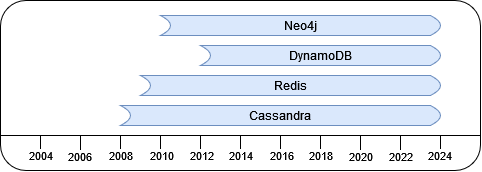
\includegraphics[width=\linewidth]{figs/lineatemporal-nosql.png}
          \vspace{-0.4cm}
          \caption{Línea temporal de tecnologías.}
    \end{minipage}
    \hspace{0.02\textwidth}
    \begin{minipage}{0.48\textwidth}
          \centering
          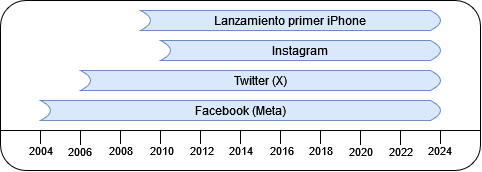
\includegraphics[width=\linewidth]{figs/lineatemporal-tecno.png}
          \vspace{-0.4cm}
          \caption{Línea temporal de sist. NoSQL.}
    \end{minipage}
    \end{figure}

    Notar el paralelismo que existe entre el surgimiento de nuevas tecnologías y el desarrollo de sistemas NoSQL.
    
    \item \textbf{NewSQL.} La quinta generación tuvo lugar a partir de la década de 2010, con una categoría emergente de bases de datos que busca ofrecer una solución que equilibre la escalabilidad con las garantías ACID\footnote{Atomocidad, Consistencia, Aislamiento y Durabilidad.}, permitiendo a las empresas aprovechar las ventajas de ambas tecnologías sin comprometer la integridad de sus datos.
\end{enumerate}

\vspace{0.2cm}

El modelo relacional fue, por muchos años, la elección por defecto para implementar bases de datos. Pero a día de hoy, las bases de datos NoSQL están ganando terreno debido a las exigencias de las aplicaciones del siglo XXI. Igualmente, la tecnología más utilizada depende del caso de uso específico. En general, NoSQL es más popular para aplicaciones web a gran escala con grandes conjuntos de datos, mientras que SQL es más popular para aplicaciones transaccionales que requieren ACID.

También hay que tener en cuenta las tendencias. Algunas bases de datos ofrecen características de ambos mundos; otras, como las NewSQL, que buscan ofrecer escalabilidad horizontal con garantías ACID.

\section{Conceptos Básicos}\label{sec3}

\subsection{Bases de datos NoSQL}\label{sec31}

La definición más simple de una Base de Datos NoSQL es: ``\textit{Una base de datos que difiere del modelo relacional}''\cite{fund}, esto significa que no se basan en una estructura rígida de tablas y relaciones, lo que les permite adaptarse mejor a las necesidades de aplicaciones específicas. Esta definición abarca una amplia gama de modelos de datos, es por esto que además presentan las siguientes características:

\begin{itemize}
    \item Pueden correr fácilmente en clusters sin SPOFs\footnote{\textit{Single Point of Failure}: Punto de un sistema que si falla, causará una interrupción o fallo en todo el sistema.}, lo que les da la posibilidad de tener un escalado horizontal (\textit{Scale-out}).
    
    \item Operan sin un esquema fijo, permitiendo agregar campos a los registros cuando el sistema está operativo.
    
    \item Siguen el principio \textbf{BASE} (\textbf{B}asically \textbf{A}vailable, \textbf{S}oft State, \textbf{E}ventually Consistent). Sacrifican la consistencia por consistencia eventual, tolerancia a particiones y disponibilidad.
    
    \item Hacen incapié en el desempeño y la flexibilidad sobre la potencia de modelización y las consultas complejas.
    
    \item Usualmente son nuevas y de software libre.
\end{itemize}

Estos modelos no apuntan a ser un reemplazo de las bases de datos relacionales, pero dan otra opción a nuevos desarrollos.

Además, es importante tener en cuenta que la mejora en el rendimiento se nota con volúmenes grandes de información, lo cual podremos ver en secciones siguientes.

Muchas implementaciones NoSQL tienen lenguajes de consulta menos potentes que los modelos relacionales, ya que no se requiere una alta potencia. Es por esto que estos sistemas suelen proveer un conjunto de funciones/operaciones mas pequeño y sencillo que el que proveen los modelos SQL. 

En muchos casos, dichas operaciones son llamadas \textbf{CRUD} que viene de:

\begin{enumerate}
    \item \textit{\textbf{C}reate} (Crear)
    \item \textit{\textbf{R}ead} (Leer)
    \item \textit{\textbf{U}pdate} (Actualizar)
    \item \textit{\textbf{D}elete} (Eliminar)
\end{enumerate}

Y en algunos casos (si la operación está definida) se incluye la letra \textbf{S} al principio (\textbf{SCRUD}), proveniente de \textit{\textbf{S}earch} (Buscar).

Además de la simplificación en el lenguaje de consulta, estos modelos también simplifican la modelización de datos. Permiten datos semi-estructurados, esto significa que el sistema de almacenamiento de datos no requiere una estructura estricta para todos los datos que almacena. Puede manejar datos que no se ajustan completamente a un esquema predefinido, por lo que permiten agregar registros \textit{on-the-fly}\footnote{``Sobre la marcha.''}. Además, permiten especificar esquemas parciales, lo que significa que se puede definir solo una parte de la estructura de los datos, lo que puede mejorar la eficiencia del almacenamiento al no requerir la especificación completa del esquema.

Otra característica de los modelos NoSQL es que muchos proveen el almacenamiento de múltiples versiones de los registros, los cuales vienen con un \textit{timestamp} asociado, que indica cuando se creó/actualizó el dato. Esto permite rastrear los cambios realizados en los datos y proporciona una visión histórica de cómo han evolucionado. Este historial, en muchos casos, ya viene implementado y se realiza automáticamente.

\subsection{Sistemas Distribuidos}\label{sec32}

Como se mencionó en la sección \ref{sec31}, una de las características de las implementaciones del modelo NoSQL es que pueden correr fácilmente en sistemas distribuidos. Estos sistemas tienen la posibilidad de escalar horizontalmente, lo que implica agregar más instancias (nodos) para aumentar la capacidad del sistema. Es por esto que estos sistemas ofrecen alto rendimiento y disponibilidad, soportan paralelismo y estructuras distribuidas.

Es por esto que es importante tener en cuenta conceptos de sistemas distribuidos tales como: 

\begin{enumerate}
    \item Modelos de Replicación
    \item Partición de Archivos
    \item Acceso de Datos de Alto Desempeño
    \item Conjetura de Brewer
\end{enumerate}

\subsubsection{Modelos de Replicación}\label{sec321}

El escalado horizontal generalmente se realiza cuando el sistema está operativo, lo que implica que se necesitan técnicas para distribuir los datos existentes entre los nuevos nodos sin interrumpir al sistema.

Los dos principales modelos utilizados son el de \textit{Maestro-Esclavo} y el de \textit{Maestro-Maestro}.

\vspace{0.1cm}

\noindent
\textbf{Modelo Maestro-Esclavo.} El servidor \textbf{maestro} es el nodo principal en el sistema. Es el responsable de aceptar escrituras (actualizaciones, inserciones y eliminaciones) en la base de datos. Cualquier cambio realizado en el maestro es replicado en los esclavos.

Los servidores \textbf{esclavos} son nodos secundarios que se sincronizan con el maestro para mantener una copia exacta de los datos. Los esclavos solo pueden aceptar lecturas de la base de datos. Los cambios realizados en el maestro se replican de forma asíncrona o síncrona en los esclavos para mantenerlos actualizados.

La replicación de datos se produce desde el maestro a los esclavos. 

Hay dos tipos principales de replicación:

\begin{enumerate}
    \item \textbf{Replicación síncrona.} En este caso, el maestro espera a que todos los esclavos confirmen que han recibido y aplicado los cambios antes de confirmar la transacción al cliente. Esto garantiza que todos los esclavos tengan una copia exacta de los datos en todo momento, pero puede introducir latencia en las operaciones de escritura.
    
    \item \textbf{Replicación asíncrona.} El maestro envía los cambios a los esclavos de forma asíncrona, lo que significa que el maestro no espera una confirmación de los esclavos antes de confirmar la transacción al cliente. Esto puede mejorar el rendimiento y la escalabilidad, pero existe el riesgo de que los esclavos se retrasen en la aplicación de los cambios, lo que podría causar inconsistencias temporales en los datos.
\end{enumerate}

\begin{wrapfigure}{r}{0.42\textwidth}
    \centering
    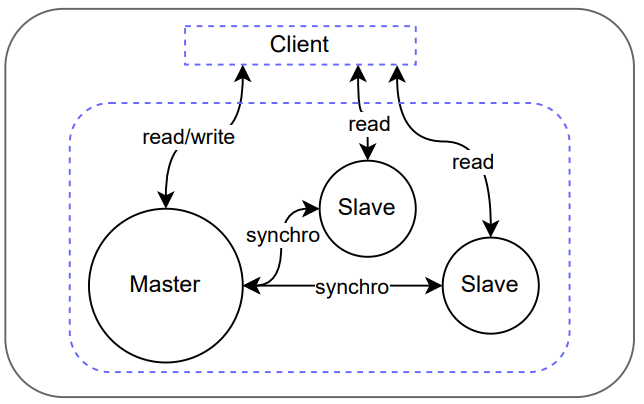
\includegraphics[width=0.42\textwidth]{figs/maestro-esclavo.png}
    \caption{Modelo Maestro-Esclavo.}
\end{wrapfigure}

Al implementar este modelo, se pueden lograr varios beneficios, como:

\begin{enumerate}
    \item \textbf{Escalabilidad.} Los esclavos pueden manejar consultas de lectura, distribuyendo la carga de trabajo y mejorando el rendimiento del sistema.

    \item \textbf{Disponibilidad.} Si el maestro falla, uno de los esclavos puede promoverse para convertirse en el nuevo maestro, manteniendo así la disponibilidad del sistema.

    \item \textbf{Tolerancia a fallos.} Al mantener copias redundantes de los datos en los esclavos, el sistema puede tolerar la pérdida de uno o varios nodos sin perder acceso a los datos.
\end{enumerate}

\vspace{0.1cm}

\noindent
\textbf{Modelo Maestro-Maestro.} En este modelo todos los nodos en el sistema son tanto \textbf{maestros} como \textbf{esclavos}. Esto significa que cada nodo puede aceptar escrituras y propagarlas a otros nodos en el sistema, así como también recibir cambios de otros nodos y aplicarlos localmente.

\begin{wrapfigure}{r}{0.42\textwidth}
    \centering
    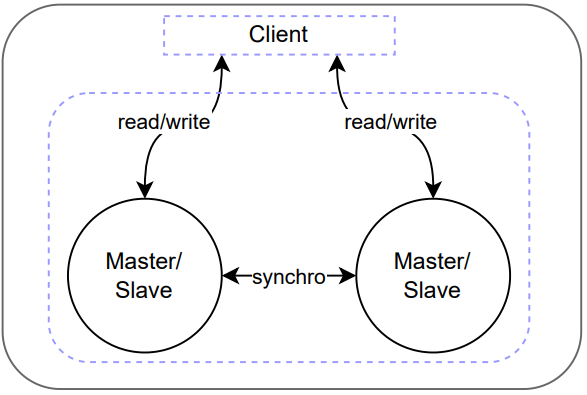
\includegraphics[width=0.42\textwidth]{figs/maestro-maestro.png}
    \caption{Modelo Maestro-Maestro.}
\end{wrapfigure}

La replicación de datos es bidireccional. Esto significa que los cambios realizados en cualquier nodo se replican en todos los demás nodos en el sistema. Cada nodo es responsable de mantener una copia exacta de los datos y asegurarse de que todos los demás nodos estén sincronizados.

Una consideración importante en este modelo son los conflictos de escritura, que pueden ocurrir cuando dos nodos intentan actualizar la misma porción de datos al mismo tiempo. Para abordar este problema, se requieren mecanismos de resolución de conflictos, que pueden incluir la implementación de reglas de prioridad, estampados de tiempo o la intervención manual.

Al implementar un modelo Maestro-Maestro, se pueden lograr varios beneficios, incluyendo:

\begin{enumerate}
    \item  \textbf{Alta disponibilidad.} Debido a que todos los nodos pueden aceptar escrituras, el sistema puede continuar funcionando incluso si uno de los nodos falla.

    \item \textbf{Escalabilidad horizontal.} Se pueden agregar más nodos al sistema para manejar cargas de trabajo crecientes, lo que mejora el rendimiento y la capacidad del sistema.

    \item \textbf{Tolerancia a fallos.} Si un nodo falla, los demás nodos pueden seguir aceptando escrituras y manteniendo la disponibilidad del sistema.
\end{enumerate}

\subsubsection{Partición de Archivos}\label{sec322}

Otra característica a considerar es la partición de archivos. En el contexto de sistemas distribuidos, la partición de archivos se refiere a la división de los datos en fragmentos más pequeños y manejables que se distribuyen entre múltiples nodos en un clúster. Es un concepto importante en sistemas distribuidos para mejorar el rendimiento y la escalabilidad al distribuir la carga de trabajo entre varios nodos.

Este concepto permite distribuir los datos entre múltiples nodos, lo que puede mejorar el rendimiento al permitir que las consultas se distribuyan entre varios nodos y se ejecuten en paralelo.

Puede aumentar la resiliencia del sistema al distribuir los datos de manera redundante entre múltiples nodos. Si un nodo falla, los datos aún estarán disponibles en otros nodos del clúster, lo que ayuda a mantener la disponibilidad del sistema.

La combinación de partición de los registros de archivos y la replicación de los datos cooperan para mejorar el balance de carga de los nodos y su disponibilidad.

\subsubsection{Acceso de Datos de Alto Desempeño}\label{sec323}

Como hemos visto en secciones anteriores, los sistemas cada vez manejan mayor cantidad de información. Es por esto que generalmente, se necesita encontrar un registro particular entre millones. Aquí entra en juego el acceso de datos de alto desempeño (\textit{High Performance Data Access}). El \textbf{HPDA}, por sus siglas en inglés, se refiere a la capacidad de un sistema para acceder y manipular grandes volúmenes de datos de manera rápida y eficiente.

Para lograr esto, se suelen utilizar técnicas de \textit{hashing} o particionado de rango sobre las claves de los objetos.

En el \textit{hashing}, se aplica una función de \textit{hash} $h$ a la clave $K$ del objeto para determinar su ubicación en el sistema distribuido. La aplicación $h(K)$ es la que da la ubicación del objeto con clave $K$. Esto permite una distribución uniforme de los datos y facilita la búsqueda eficiente del objeto en el sistema distribuido.

En el particionado de rango, se asignan los objetos a ubicaciones en función de un rango de valores de clave. Por ejemplo, una ubicación $u$ podría tener los objetos cuyas claves $K$ estén en el rango $Ku_{min} \leq K \leq Ku_{max}$. Esto puede simplificar la distribución de datos en ciertos escenarios donde hay cierta correlación entre los valores de clave y su ubicación física en el sistema.

Ambas técnicas pueden utilizarse para distribuir de manera efectiva los datos entre múltiples nodos en un sistema distribuido. Además, dependiendo de los requisitos específicos de la aplicación y el tipo de consultas que se deseen realizar, también se pueden aplicar otras técnicas de indexación para optimizar el acceso a los objetos. Estas técnicas pueden incluir la creación de índices secundarios, árboles B+, estructuras de datos \textit{hash} adicionales, entre otras.

\subsubsection{Conjetura de Brewer}\label{sec324}

Como la mayoría de las implementaciones del modelo NoSQL soportan entornos distribuidos, es importante tener en cuenta la \textbf{Conjetura de Brewer}, también conocida como Teorema CAP. 

Las siglas \textbf{CAP} vienen de:

\begin{itemize}
    \item \textbf{C} de \textit{\textbf{C}onsistency} (Consistencia), se refiere a la consistencia de los valores en diferentes copias del mismo dato. 
    
    \item \textbf{A} de \textit{\textbf{A}vailability} (Disponibilidad), es decir, cualquier petición recibe una respuesta no errónea, pero sin la garantía de que contenga la escritura más reciente.

    \item \textbf{P} de \textit{\textbf{P}artition Tolerance} (Tolerancia a Particiones), es decir, el sistema sigue funcionando incluso si un número arbitrario de mensajes son descartados (o retrasados) entre nodos de la red.
\end{itemize}

Según esta conjetura, en un sistema distribuido solo se pueden cumplir dos de estas tres propiedades simultáneamente. Es por esto que es importante elegir cuáles dos propiedades son más importantes según las necesidades del sistema y las expectativas del usuario.

En los modelos relacionales, los cuáles deben cumplir ACID, es importante que se garantice la consistencia. Pero en los sistemas NoSQL, es aceptable garantizar un nivel de consistencia menor, sacrificando esta propiedad para cumplir en mayor medida la disponibilidad y la tolerancia a particiones.

\subsection{SQL versus NoSQL}\label{sec33}

Como se vió en secciones anteriores, las bases de datos SQL y NoSQL difieren en varios aspectos clave. Se enuncian algunas de sus principales diferencias:

\begin{itemize}
    \item \textbf{Modelo de Datos}

    Los sistemas SQL utilizan el modelo de datos relacional, el cuál tiene un estándar, basado en tablas con filas y columnas. Se utiliza un esquema fijo y las relaciones entre las tablas están definidas mediante claves primarias y foráneas.

    Los sistemas NoSQL pueden utilizar varios modelos, los cuales pueden ser más flexibles y adaptarse mejor a ciertos tipos de datos no estructurados o semiestructurados.

    \item \textbf{Escalabilidad}
    
    Tradicionalmente, las bases de datos SQL escalan verticalmente, lo que significa que se aumenta la capacidad de hardware de un solo servidor para manejar una carga de trabajo mayor. 
    
    Suelen escalar horizontalmente, lo que implica distribuir la carga de trabajo entre varios servidores o nodos en un clúster. Esto permite una escalabilidad más fácil y flexible para grandes volúmenes de datos y cargas de trabajo distribuidas.
    
    \item \textbf{Consistencia}
    
    Las bases de datos SQL siguen el principio ACID cuando son implementadas en Sistemas Distribuidos, lo que garantiza la consistencia de los datos en todas las transacciones. Es decir, todos los nodos de la red, deben tener sus datos sincronizados previo a finalizar la transacción.
    
    La mayoría de las bases de datos NoSQL priorizan la disponibilidad y la tolerancia a particiones sobre la consistencia, siguiendo el principio BASE. Esto significa que los datos pueden estar en un estado no consistente temporalmente, pero se espera que converjan hacia un estado consistente en algún momento.

    \item \textbf{Query Language}

    Las bases de datos SQL se caracterizan por tener un lenguaje de consulta poderoso (justamente, el lenguaje SQL), el cuál permite a los usuarios realizar consultas complejas. El lenguaje SQL está basado en el Álgebra relacional y el Cálculo relacional de Tuplas.

    Las bases de datos NoSQL no siguen un lenguaje estándar, cada implementación tiene su propio lenguaje de consulta, aunque implementaciones bajo una misma clasificación tienenden a coincidir en lo que ofrecen. Estos lenguajes generalmente son menos complejos y potentes que el lenguaje SQL.

    
\end{itemize}

\section{Modelos de Datos NoSQL}\label{sec4}

Existe una amplia variedad de modelos de datos NoSQL, cada uno con sus propias características, ventajas y desventajas. Entre los más conocidos encontramos:

\begin{enumerate}
    \item \textbf{Clave-Valor}
    \item \textbf{Columnar}
    \item \textbf{Documental}
    \item \textbf{en Grafo}

    \vspace{0.1cm}
    
    \noindent
    Adicionalmente, se agregan algunas categorías para clasificar implementaciones que no se adaptan a las mencionadas anteriormente, y también otras que están disponibles incluso desde antes de que los sistemas NoSQL se volvieran ampliamente utilizados, por ejemplo:

    \vspace{0.1cm}
        
    \item \textbf{Sistemas NoSQL Hibridos.} Sistemas que tienen características de dos o más de las cuatro categorías anteriores.
    \item \textbf{Bases de Datos de Objetos} 
    \item \textbf{Bases de Datos XML}
\end{enumerate}

No se va a profundizar sobre estas últimas tres categorías.

\subsection{Clave-Valor}\label{sec41}

Como indica su nombre, este modelo almacena pares del tipo (\textit{key}, \textit{value}) de la misma manera que lo hacen los mapas (o \textit{tablas hash}). Está basado sobre el acceso rápido por la clave a su valor asociado; dicho valor puede ser un registro, un objeto, un documento o cualquier estructura de datos más compleja. Para el modelo, los valores son objetos oscuros, que no sabe interpretar. Su simplicidad destaca por la facilidad a la hora de particionar los datos y las consultas eficientes de datos, lo que se refleja en la alta escalabilidad horizontal de esta arquitectura \cite{surv}.

El acceso rápido a valores es logrado con métodos de búsqueda por clave eficientes utilizando \textit{Tablas Hash Distribuidas}(DHTs) y/o árboles \textit{Log Structured-Merge}\cite{Atzeni2016DataMI}

Se puede decir que es el modelo de datos NoSQL más simple desde el punto de vista de su uso, debido a que su interfaz consta solo de tres operaciones que el cliente puede utilizar:

\begin{itemize}
    \item \textbf{get.} Esta operación recibe una \textit{key} y devuelve su \textit{value} asociado, si es que la \textit{key} recibida existe. Caso contrario, se lanza un error.
    
    \item \textbf{set.} Esta operación recibe un par (\textit{key}, \textit{value}) el cuál inserta en la base de datos. Si ya existe la \textit{key} ingresada en el modelo, el comportamiento depende de cada implementación, pero esencialmente pueden existir dos posibles comportamientos:

    \begin{enumerate}
        \item \textbf{Sobrescritura del Valor.} Se sobreescribe el valor anterior asociado a la \textit{key} recibida por el nuevo valor.
        \item \textbf{Error de Duplicación de Clave.} Se lanza una excepción indicando que ya existe la clave en la base de datos.
    \end{enumerate}

    También en algunas implementaciones este comportamiento es configurable.
    
    \item \textbf{remove.} Esta operación recibe una \textit{key} y elimina su \textit{value} asociado, si es que la \textit{key} recibida existe. Caso contrario, se lanza un error.
\end{itemize}

El modelo de bases de datos clave-valor ofrece varias ventajas significativas. Una de las principales es su flexibilidad, ya que no existe una estructura de tabla rígida, lo que permite esquemas flexibles que se adaptan fácilmente a los cambios en los datos. Los campos pueden añadirse o modificarse dinámicamente sin afectar la base de datos existente.

Estas bases de datos también son altamente escalables. Funcionan en clústeres, lo que facilita la adición de nodos para manejar grandes volúmenes de datos. Esta capacidad de trabajar en clústeres permite la replicación de datos en varios nodos, asegurando una alta disponibilidad y evitando la pérdida de datos.

La velocidad de procesamiento es otra ventaja importante. Los motores de procesamiento en paralelo y las arquitecturas en clústeres reducen los tiempos de consulta y mejoran la velocidad de escritura y lectura. Esto hace que las bases de datos clave-valor sean ideales para aplicaciones que requieren un rendimiento rápido y eficiente.

Algunos ejemplos de estos modelos de datos son: \textit{CouchDB}, \textit{Project Voldemort}, \textit{Redis} y \textit{DynamoDB} de Amazon.

\subsubsection{Redis}\label{sec411}

\textbf{Redis} que significa ``\textbf{RE}mote \textbf{DI}ctionary \textbf{S}erver'', como se menciona en su documentación\cite{redis}, es una base de datos en memoria de código abierto rápida y versátil, de código abierto. Diseñado como un almacén de estructuras de datos en memoria, Redis es conocida por su velocidad y capacidad para manejar una variedad de casos de uso.

Proporciona estructuras de datos como \textit{strings} (valor más simple), \textit{hashes}, listas, conjuntos, conjuntos ordenados con consultas de rango, mapas de bits, hyperloglogs, índices geoespaciales y \textit{streams}. Se pueden realizar operaciones \textbf{atómicas} sobre estas estructuras, como agregar un caracter al final de un \textit{string}; incrementar el valor en un \textit{hash}; agregar un elemento a una lista; calcular la intersección, unión y diferencia de conjuntos; u obtener el miembro con el ranking más alto en un conjunto ordenado.

Redis tiene replicación de datos incorporada, scripting \textit{Lua}, evicción \textit{LRU}, transacciones y diferentes niveles de persistencia en disco, y proporciona alta disponibilidad a través de \textit{Redis Sentinel} y particionamiento automático con \textit{Redis Cluster}.

Además soporta la replicación asíncrona, con sincronización rápida y no bloqueante, y reconexión automática con resincronización parcial en caso de división de red.

Para lograr un rendimiento óptimo, Redis trabaja con un conjunto de datos en memoria. Dependiendo el caso de uso. Puede persistir la información ya sea mediante el volcado periódico de datos en el disco o mediante el agregado de cada comando a un \textit{log}\footnote{Se refiere a la grabación secuencial de todos los acontecimientos que afectan a un proceso particular en un sistema.} en el disco. También se puede desactivar la persistencia si solo se necesita una caché en memoria.

Redis ofrece más de \textbf{400} operaciones en su interfaz, se analizan las más utilizadas, que se corresponden con las operaciones definidas en la teoría, implementadas sobre distintos tipos de datos.

\begin{enumerate}
    \item \textbf{SET.} Agrega un par $(key, value)$, donde el valor es de tipo \textit{string}, con una complejidad temporal de $\mathcal{O}(1)$\footnote{Notación \href{https://en.wikipedia.org/wiki/Big_O_notation}{\textit{Big-O}.}}. 
    
    Si ya existe la $key$ recibida, su valor se sobreescribe por el nuevo valor recibido.

    \begin{verbatim}
    redis> SET subject1 "Base de Datos Avanzadas"
    OK
    redis> SET subject2 "Verificación con F*"
    OK
    redis>
    \end{verbatim}

    \vspace{-0.5cm}
    
    \item \textbf{GET.} Obtiene el valor de una $key$ con una complejidad temporal de $\mathcal{O}(1)$. Solo se puede utilizar con valores de tipo \textit{string}.

    \begin{verbatim}
    redis> GET subject1
    "Bases de Datos Avanzadas"
    redis> GET nonexistingsubject
    (nil)
    redis>
    \end{verbatim}

    \vspace{-0.5cm}
    
    \item \textbf{DEL.} Elimina una o más claves, con una complejidad temporal de $\mathcal{O}(N)$ donde $N$ es el número de claves a eliminar. Si una $key$ a eliminar tiene un valor distinto a un \textit{string}, entonces la complejidad temporal para esta clave individualmente es $\mathcal{O}(M)$ donde $M$ es el número de elementos en la lista, conjunto, conjunto ordenado o \textit{hash}. En caso de que el valor de la clave sea un string, la complejidad es $\mathcal{O}(1)$

    Si alguna $key$ recibida no existe, se la ignora.

    \begin{verbatim}
    redis> DEL subject1 subject2 nonexistingsubject
    (integer) 2
    redis>
    \end{verbatim}

    \vspace{-0.5cm}
    
    % \item \textbf{INCR.} Incrementa el valor asociado a la $key$ recibida en uno, con una con una complejidad temporal de $\mathcal{O}(1)$. Esta operación esta limitada a enteros con signo de 64 bits.

    % Si el valor de la $key$ no es un entero con signo de 64 bits, o no se puede representar mediante este tipo, devuelve un error.

    % \begin{verbatim}
    % redis> SET counter "0"
    % redis> INCR counter
    % (integer) 1
    % redis>
    % \end{verbatim}

    % \vspace{-0.5cm}
    
    % \item \textbf{DECR.} Decrementa el valor asociado a la $key$ recibida en uno, con una con una complejidad temporal de $\mathcal{O}(1)$. Como la operación \textbf{INCR}, esta operación esta limitada a enteros con signo de 64 bits.

    % Si el valor de la $key$ no es un entero con signo de 64 bits, o no se puede representar mediante este tipo, devuelve un error.
    
    % \begin{verbatim}
    % redis> DECR counter
    % (integer) 0
    % redis>
    % \end{verbatim}
        
    \item \textbf{HSET.} Asigna al \textit{hash} recibido, los pares $(key, value)$ recibidos. Sobreescribe el valor de una $key$ recibido, si este ya existía en el \textit{hash}. Esta operación tiene una complejidad temporal de $\mathcal{O}(1)$ por cada par añadido, es decir, $\mathcal{O}(N)$ para añadir $N$ pares al \textit{hash}.

    \begin{verbatim}
    redis> HSET myhash word1 "Bases" word2 "D"
    (integer) 2
    redis> HSET myhash word3 "Datos" word4 "NoSQL" word2 "De"
    (integer) 2
    redis> HGET myhash word3
    "Datos"
    \end{verbatim}

    \vspace{-0.5cm}
    
    \item \textbf{HGET.} Obtiene el valor de un campo en un \textit{hash} con una complejidad temporal de $\mathcal{O}(1)$.

    \begin{verbatim}
    redis> HGET myhash word2
    "De"
    redis> HGET myhash nonexistingword
    (nil)
    redis>
    \end{verbatim}

    \vspace{-0.5cm}
        
    \item \textbf{LPUSH.} Inserta todos los valores recibidos en la cabeza de la lista relacionada a la $key$ recibida. Esto lo hace con una complejidad temporal de $\mathcal{O}(N)$ donde $N$ es la cantidad de valores a agregar. Si la $key$ recibida no existe, se crea una lista vacia, y se agregan los valores recibidos a ella. 
    
    Si el valor de la $key$ no es una lista, se devuelve un error.

    \begin{verbatim}
    redis> LPUSH mylist "NoSQL"
    redis> LPUSH mylist "Datos" "De" "Bases"
    redis> LRANGE mylist 0 2
    1) "Bases"
    2) "De"
    3) "Datos"
    redis>
    \end{verbatim}

    \vspace{-0.5cm}

    \item \textbf{LPOP.} Elimina y retorna los $N$ primeros elementos de la lista relacionada a la $key$ recibida. $N$ también se pasa por parámetro. Esta operación tiene una complejidad temporal de $\mathcal{O}(N)$, donde $N$ es el parámetro recibido. Si no se pasa el parámetro $N$, por default el valor es 1.

    Si el valor de la $key$ no es una lista, se devuelve un error.
    
    \begin{verbatim}
    redis> LPOP mylist 2
    1) "Bases"
    2) "De"
    redis> LPOP mylist
    "Datos"
    redis>
    \end{verbatim}

    \vspace{-0.5cm}
    
    \item \textbf{RPUSH.} Funciona como \textbf{LPUSH}, pero agregando los elementos en la cola de la lista. Esto lo realiza con una complejidad temporal de $\mathcal{O}(N)$ donde $N$ es la cantidad de valores a agregar.

    Si el valor de la $key$ no es una lista, se devuelve un error.

    \begin{verbatim}
    redis> RPUSH mylist2 "Bases"
    redis> RPUSH mylist2 "De" "Datos" "NoSQL"
    redis> LRANGE mylist2 0 2
    1) "Bases"
    2) "De"
    3) "Datos"
    redis>
    \end{verbatim}

    \vspace{-0.5cm}
    
    \item \textbf{RPOP.} Funciona como \textbf{LPOP} pero eliminando y retornando los $N$ últimos elementos de la lista relacionada a la $key$ recibida. La complejidad temporal es la misma.

    Si el valor de la $key$ no es una lista, se devuelve un error.

    \begin{verbatim}
    redis> RPOP mylist2 2
    1) "NoSQL"
    2) "Datos"
    redis> RPOP mylist2
    "De"
    redis>
    \end{verbatim}

    \vspace{-0.5cm}
    
    \item \textbf{LRANGE.} Devuelve los elementos contenidos en el rango especificados en la lista relacionada a la $key$ recibida. Tiene una complejidad temporal de $\mathcal{O}(S + N)$ donde $S$ es la distancia desde el inicio de la lista hasta el extremo izquierdo del rango recibido (para \textit{small lists}), la distancia más corta (desde el inicio o el fin) hacia alguno de los extremos del rango recibido (para \textit{large lists}); y $N$ es la cantidad de elementos contenidos en el rango recibido.

    Si el valor de la $key$ no es una lista, se devuelve un error.
    
    \begin{verbatim}
    redis> LPUSH mylist3 "a" "b" "c"
    redis> LRANGE mylist3 0 0
    "a"
    redis> LRANGE mylist3 1 2
    1) "b"
    2) "c"
    redis>
    \end{verbatim}

    \vspace{-0.5cm}
    
    % \item \textbf{SADD.} Agrega los elementos especificados al conjunto relacionado a la $key$ recibida. Tiene una complejidad temporal de $\mathcal{O}(N)$ donde $N$ es la cantidad de elementos en el conjunto. 
    
    % Si se agrega un miembro que ya está contenido en el conjunto, este es ignorado.
    
    % Si no existe un conjunto relacionado a la $key$ recibida, se crea uno vacío y se agregan los valores especificados.

    % En caso de que la $key$ recibida exista, y no esté relacionada a un conjunto, devuelve un error.

    % \begin{verbatim}
    % redis> SADD myset "Bases" "De"
    % (integer) 2
    % redis> SADD myset "Datos" "Avanzadas"
    % (integer) 2
    % redis> SADD myset "Bases"
    % (integer) 0
    % redis> SMEMBERS myset
    % 1) "Bases"
    % 2) "De"
    % 3) "Datos"
    % 4) "Avanzadas"
    % redis>
    % \end{verbatim}

    % \vspace{-0.5cm}
    
    % \item \textbf{SMEMBERS.} Retorna todos los miembros del conjunto asociado a la $key$ recibida. Tiene una complejidad temporal de $\mathcal{O}(N)$ donde $N$ es la cantidad de elementos del conjunto.

    % En caso de que el valor asociado a la $key$ recibida no sea un conjunto, devuelve un error.

    % Si no existe un conjunto relacionado a la $key$ recibida, se crea uno vacío y se agregan los valores especificados.

    % En caso de que la $key$ recibida exista, y no esté relacionada a un conjunto, devuelve un error.

    % \begin{verbatim}
    % redis> SADD myset2 "b" "c"
    % (integer) 2
    % redis> SADD myset2 "a"
    % (integer) 1
    % redis> SADD myset2 "a"
    % (integer) 0
    % redis> SMEMBERS myset
    % 1) "b"
    % 2) "c"
    % 3) "a"
    % redis>
    % \end{verbatim}
        
    \item \textbf{ZADD.} Funciona como \textbf{SADD} pero sobre conjuntos ordenados. Cada elemento recibido tiene asociado un \textit{score} el cuál va a indicar su posición en el conjunto. Tiene una complejidad temporal de $\mathcal{O}(log(N))$ donde $N$ es la cantidad de elementos en el conjunto. 

    Si se agrega un miembro que ya está contenido en el conjunto, este es ignorado, al menos que se le modifique el \textit{score}, en ese caso, se sobreescribe dicho valor, actualizando así su posición en el conjunto.
    
    Si no existe un conjunto ordenado relacionado a la $key$ recibida, se crea uno vacío y se agregan los valores especificados.

    En caso de que la $key$ recibida exista, y no esté relacionada a un conjunto ordenado, devuelve un error.
    
    \begin{verbatim}
    redis> ZADD myzset 2 "b" 3 "c"
    (integer) 2
    redis> ZADD myzset 4 "a"
    (integer) 1
    redis> ZMEMBERS myset
    1) "b"
    2) "c"
    3) "a"
    redis> ZADD myzset 1 "a"
    (integer) 0
    redis> ZMEMBERS myset
    1) "a"
    2) "b"
    3) "c"
    redis>
    \end{verbatim}

    \vspace{-0.5cm}
    
    \item \textbf{ZRANGE.} Funciona como \textbf{LRANGE} pero sobre conjuntos ordenados. Tiene una complejidad temporal de $\mathcal{O}(log(N) + M)$ donde $N$ es la cantidad de elementos en el conjunto ordenado, y $M$ es la cantidad de elementos a devolver.

    Además permite que los elementos a devolver sean ordenados según sus \textit{scores}, según el orden lexicográfico o por índice. También permite devolver los elementos de este conjunto revertidos.

    \begin{verbatim}
    redis> ZMEMBERS myset REV
    1) "c"
    2) "b"
    3) "a"
    redis> ZADD myzset 4 "a"
    (integer) 0
    redis> ZMEMBERS myset BYLEX
    1) "a"
    2) "b"
    3) "c"
    redis> ZMEMBERS myset WITHSCORES
    1) "2"
    2) "b"
    3) "3"
    4) "c"
    5) "4"
    6) "a"
    \end{verbatim}
\end{enumerate}

\vspace{-1cm}

\subsection{Columnar}\label{sec42}

Las bases de datos orientadas a columnas (también llamadas \textit{bases de datos de registros extensibles}) almacenan los datos verticalmente por columnas en lugar de horizontalmente por filas como en las bases de datos relacionales tradicionales. Esta estructura permite un acceso más eficiente a datos específicos, ya que cada columna de una tabla se almacena de forma contigua en el disco. Esto facilita la recuperación rápida de datos y la realización de operaciones analíticas sobre conjuntos de datos grandes.

No obstante, estas bases de datos también presentan algunas desventajas como por ejemplo las operaciones de escritura pueden ser más lentas debido a la necesidad de reorganizar los datos en columnas específicas.

En cuanto a las aplicaciones y casos de uso, las bases de datos columnares son especialmente adecuadas para el análisis de grandes volúmenes de datos en aplicaciones de \textit{Business Intelligence}\footnote{Proceso de recopilación, análisis y presentación de información empresarial para ayudar en la toma de decisiones estratégicas.} y análisis predictivo. Su capacidad para realizar operaciones analíticas eficientes en columnas específicas las hace ideales para aplicaciones que requieren análisis detallados y reportes de datos. Además, son ampliamente utilizadas en entornos donde se manejan datos de series temporales, como registros de transacciones financieras o datos de sensores \textit{IoT}\footnote{Internet de las Cosas. Red de dispositivos físicos conectados a Internet que intercambian datos entre sí y con otros sistemas.}.

Algunos ejemplos de bases de datos columnares son:
\begin{itemize}
    \item \textit{Apache Cassandra}: Aunque es principalmente una base de datos de clave-valor, Cassandra utiliza un modelo de almacenamiento columnar para mejorar el rendimiento de ciertas consultas.
    \item \textit{Apache HBase}: HBase es una base de datos de columnas distribuida, que almacena datos de forma columnar y permite un acceso eficiente a través de claves de fila.
    \item \textit{ClickHouse}: ClickHouse es una base de datos de análisis columnar de código abierto diseñada para consultas analíticas de alto rendimiento en grandes conjuntos de datos.
\end{itemize}

\subsubsection{HBase}\label{sec421}

\textbf{HBase} \cite{hbase} es una base de datos NoSQL distribuida y escalable, desarrollada por la \textit{Apache Software Foundation}, inspirada en el diseño del sistema Bigtable de Google. Su modelo de datos se basa en tablas similares a las de las bases de datos relacionales, pero con una estructura flexible basada en columnas. Los datos se organizan en filas indexadas por una clave única y se agrupan en familias de columnas, lo que proporciona una gran flexibilidad en la estructura de los datos. 

Internamente, HBase utiliza un modelo de datos ordenados por clave y almacena los datos en archivos HFile en el sistema de archivos \textit{Hadoop HDFS}. Utiliza un sistema de partición distribuida para dividir los datos en regiones y un sistema de replicación para garantizar la disponibilidad y la tolerancia a fallos. Además, ofrece diferentes niveles de consistencia para adaptarse a las necesidades de las aplicaciones, lo que permite a los desarrolladores equilibrar entre disponibilidad y consistencia de datos. HBase se utiliza en una variedad de aplicaciones que requieren un almacenamiento y recuperación de datos de alta velocidad, como análisis de datos en tiempo real, indexación y búsqueda de texto completo, y seguimiento de eventos, entre otros.


HBase proporciona un conjunto de comandos específicos del sistema a través del \textbf{HBase Shell}, que se utiliza para realizar diversas operaciones administrativas y de consulta. Estos comandos permiten realizar tareas como la creación y gestión de tablas, la inserción y recuperación de datos, el escaneo de tablas, entre otros. Además del HBase Shell, los desarrolladores también pueden interactuar con HBase a través de la API Java de HBase para realizar operaciones en sus aplicaciones Java.

A continuación se describen algunas operaciones comunes:

\begin{enumerate}
    \item \textbf{create}: Se utiliza para crear una nueva tabla, especificando el nombre de la tabla y las familias de columnas que contendrán los datos.
    
    \begin{verbatim}
hbase(main):001:0> create 'usuarios', 'datos_personales', 'datos_contacto'
    \end{verbatim}

    \vspace{-0.25cm}
    
    \item \textbf{put}: Se utiliza para insertar un valor en una celda de datos específica.
    \begin{verbatim}
hbase(main):002:0> put 'usuarios', '1001', 'datos_personales:nombre', 'Juan'

hbase(main):003:0> put 'usuarios', '1001', 'datos_personales:apellido', 'Pérez'

hbase(main):004:0> put 'usuarios', '1001', 'datos_contacto:email', 'juan@example.com'
    \end{verbatim}

    \vspace{-0.25cm}
    
    \item \textbf{get}: Se utiliza para recuperar todos los datos de una familia de columnas específica para una fila dada.
    \begin{verbatim}
hbase(main):005:0> get 'usuarios', '1001', {COLUMN => 'datos_personales'}
COLUMN                                CELDA
datos_personales:nombre               timestamp=1595373585200, valor=Juan
datos_personales:apellido             timestamp=1595373585355, valor=Pérez
    \end{verbatim}

    \vspace{-0.25cm}
    
    \item \textbf{delete}: Se utiliza para eliminar una celda de datos específica.
    \begin{verbatim}
hbase(main):006:0> delete 'usuarios', '1001', 'datos_contacto:email'

hbase(main):007:0> get 'usuarios', '1001'
COLUMN                                CELDA
datos_personales:nombre               timestamp=1595373585200, valor=Juan
datos_personales:apellido             timestamp=1595373585355, valor=Pérez
    \end{verbatim}

    \vspace{-0.25cm}
    
    \item \textbf{drop}: Se utiliza para eliminar una tabla por completo.
    \begin{verbatim}
hbase(main):008:0> drop 'usuarios'
    \end{verbatim}
\end{enumerate}

\vspace{-0.4cm}

Además de las operaciones básicas, HBase ofrece funcionalidades avanzadas que permiten a los usuarios realizar tareas más complejas y sofisticadas. A continuación, se presentan algunos ejemplos de estas operaciones:

\begin{enumerate}
    \item \textbf{Escaneo de Rango}: Esta sentencia escanea todas las filas de la tabla 'usuarios' con claves entre '1001' y '2000'.
    \begin{verbatim}
    hbase(main):001:0> scan 'usuarios', {STARTROW => '1001', ENDROW => '2000'}
    \end{verbatim}

    \vspace{-0.25cm}
    
    \item \textbf{Filtros de Columnas y Filas}: Esta sentencia escanea la tabla 'usuarios' y devuelve solo las columnas de la familia 'datos\_personales' donde el nombre comienza con 'Juan'.
    \begin{verbatim}
    hbase(main):002:0> scan 'usuarios', {COLUMNS => ['datos_personales'], 
        FILTER => "PrefixFilter('Juan')"}
    \end{verbatim}
    
    \vspace{-0.25cm}
    
    \item \textbf{Transacciones y Consistencia}: Recupera los datos de la fila '1001' de la tabla 'usuarios' con una consistencia fuerte.
    \begin{verbatim}
    hbase(main):003:0> get 'usuarios', '1001', CONSISTENCY => 'STRONG'
    \end{verbatim}

    \vspace{-0.25cm}
    
    \item \textbf{Replicación de Datos}: Configura la replicación de datos desde el clúster local ('1') a otro clúster remoto.
    \begin{verbatim}
    hbase(main):004:0> replication_admin.rb add_peer '1', 
        CLUSTER_KEY => 'hbase.replication.peer.clusterkey'
    \end{verbatim}

    \vspace{-0.25cm}
        
    \item \textbf{Optimización de Rendimiento}: Estas sentencias deshabilitan, modifican y vuelven a habilitar la tabla 'usuarios' para optimizar el rendimiento.
    \begin{verbatim}
    hbase(main):005:0> disable 'usuarios'
    hbase(main):006:0> alter 'usuarios', METHOD => 'table_att', 
        'MAX_FILESIZE' => '10737418240'
    hbase(main):007:0> enable 'usuarios'
    \end{verbatim}

    \vspace{-0.25cm}
    
    \item \textbf{Seguridad}: Otorga permisos de lectura y escritura al usuario 'admin' en la tabla 'usuarios' para garantizar la seguridad de los datos.
    \begin{verbatim}
    hbase(main):009:0> grant 'admin', 'RW', 'usuarios'
    \end{verbatim}
\end{enumerate}

\vspace{-0.7cm}

\subsection{Documental}\label{sec43}

Las bases de datos documentales son un tipo de sistema de gestión de bases de datos diseñadas para el almacenamiento y gestión de datos en forma de documentos. A diferencia de las bases de datos relacionales, donde los datos se organizan en tablas con filas y columnas, las bases de datos documentales almacenan datos en documentos individuales que pueden ser estructurados o semi-estructurados, como archivos JSON o XML.

El modelo de datos documental es altamente flexible y puede adaptarse fácilmente a cambios en la estructura de los datos sin necesidad de modificar el esquema de la base de datos. Cada documento puede contener cualquier cantidad de campos de datos, lo que permite una representación variada de la información.

Los nombres de los elementos de datos pueden extraerse desde la descripción misma de los documentos en la colección. Además, los usuarios pueden requerir que el sistema cree índices sobre algunos de los elementos de datos para mejorar el rendimiento de las consultas.

Las bases de datos documentales son especialmente adecuadas para aplicaciones donde los datos tienen una estructura flexible y variable, como el contenido web, el análisis de registros y la gestión de datos de productos.

\textit{MongoDB} y \textit{CouchDB} son sistemas de gestión de bases de datos documentales que utilizan un modelo de datos basado en documentos JSON. \textit{MongoDB} es conocido por su capacidad de escalar horizontalmente y ofrece opciones avanzadas de replicación y consulta, mientras que \textit{CouchDB} es más simple en cuanto a replicación y consulta, pero puede ser más adecuado para cargas de trabajo menos intensivas.

\subsubsection{MongoDB}\label{sec431}

\textbf{MongoDB}\cite{mongodb} es una base de datos NoSQL de código abierto, orientada a documentos y altamente escalable. Desarrollada por MongoDB Inc., MongoDB utiliza un modelo de datos flexible basado en documentos BSON (Binary JSON), lo que permite almacenar datos de forma más natural y jerárquica que las bases de datos relacionales tradicionales.

Esta utiliza un enfoque de almacenamiento orientado a documentos, donde cada registro en una colección es un documento JSON que puede contener datos con una estructura diferente. Esto proporciona una gran flexibilidad en el diseño de esquemas y permite almacenar datos heterogéneos en la misma colección.

Internamente, almacena los datos en un formato binario eficiente llamado BSON y utiliza un sistema de almacenamiento basado en archivos de mapeo directo (MMAP) o un motor de almacenamiento basado en árboles de búsqueda (WiredTiger) para administrar los datos en disco.

MongoDB maneja la replicación a través de sus conjuntos de réplicas para garantizar la alta disponibilidad de los datos. Esto asegura que incluso en caso de falla de un nodo, los datos seguirán estando disponibles y accesibles.

En lugar de almacenar todos los datos en un solo servidor, MongoDB distribuye los datos en clústeres de servidores llamados fragmentos. Cada fragmento contiene una parte del conjunto de datos total y MongoDB se encarga de enrutar las consultas a los fragmentos correspondientes. Esto permite a MongoDB manejar grandes volúmenes de datos y aumentar la capacidad de almacenamiento y el rendimiento de manera lineal a medida que se agregan más servidores al clúster.

MongoDB ofrece un lenguaje de consulta poderoso y flexible que permite realizar una variedad de operaciones, incluyendo consultas ad hoc, agregaciones, indexación y más. Utiliza una interfaz de cliente basada en JSON y proporciona controladores oficiales para varios lenguajes de programación, incluyendo Python, Java, Node.js y C\#.

A continuación, se muestran algunos ejemplos de operaciones comunes:

\begin{enumerate}
    \item \textbf{Insertar un documento}: Se utiliza para agregar un nuevo documento a una colección.

    \begin{multicols}{2}
        \begin{verbatim}
    db.users.insertOne({
        name: "John Doe",
        age: 30,
        email: "john@example.com"
    })
        \end{verbatim}
    
        \columnbreak
        
        \begin{verbatim}
    db.users.insertMany([
      { name: "Alice", age: 25 },
      { name: "Bob", age: 30 },
      { name: "Charlie", age: 50 }
    ])
        \end{verbatim}
    \end{multicols}
    
    \vspace{-0.25cm}
    
    \item \textbf{Consultar documentos}: Se utiliza para recuperar documentos que coincidan con ciertos criterios de búsqueda.
    
    \begin{verbatim}
    db.users.find({ age: { $gt: 25 } })
    \end{verbatim}

    \vspace{-0.25cm}
    
    \item \textbf{Actualizar documentos}: Se utiliza para modificar los valores de campos en un documento existente.

    \begin{multicols}{2}
        \begin{verbatim}
    db.users.updateOne(
        { name: "John Doe" },
        { $set: { age: 35 } }
    )
        \end{verbatim}
    
        \columnbreak
        
        \begin{verbatim}
    db.users.updateMany(
        { status: "active" }, 
        { $set: { status: "inactive" } }
    )
        \end{verbatim}
    \end{multicols}

    \vspace{-0.4cm}
    
    \item \textbf{Eliminar documentos}: Se utiliza para eliminar documentos que coincidan con ciertos criterios de búsqueda.
    
    \begin{verbatim}
    db.users.deleteOne({ name: "John Doe" })
    db.users.deleteMany({ age: { $gt: 40 } })
    \end{verbatim}

    \vspace{-0.25cm}
        
    \item \textbf{Contar documentos}: Esta operación cuenta el número total de documentos que coinciden con los criterios de búsqueda especificados.
    
    \begin{verbatim}
    db.users.countDocuments({ age: { $lt: 30 } })
    \end{verbatim}

    \vspace{-0.25cm}
        
    \item \textbf{Valores Distintos}: Esta operación devuelve un array de valores distintos para un campo específico en la colección que coincida con los criterios de búsqueda especificados.
    
    \begin{verbatim}
    db.users.distinct("city", { country: "USA" })
    \end{verbatim}

    \vspace{-0.25cm}
    
    \item \textbf{Agregar datos}: Esta operación se utiliza para realizar operaciones de agregación en los documentos de una colección, como sumar, contar o agrupar datos.
    
    \begin{verbatim}
    db.sales.aggregate([
      { $match: { status: "completed" } },
      { $group: { _id: "$product", totalAmount: { $sum: "$amount" } } }
    ])
    \end{verbatim}
\end{enumerate}

\vspace{-0.25cm}

MongoDB es ampliamente utilizado por empresas de todos los tamaños y en una variedad de sectores, incluyendo tecnología, finanzas, comercio electrónico y más. Algunas de las empresas que utilizan MongoDB incluyen \textit{LinkedIn, eBay, Toyota, Uber}, entre otras.

MongoDB Inc. ofrece servicios y herramientas adicionales, como \textit{MongoDB Atlas}, un servicio de base de datos en la nube completamente administrado, \textit{MongoDB Compass}, una interfaz gráfica de usuario para MongoDB, y \textit{MongoDB University}, una plataforma de aprendizaje en línea para desarrolladores.


\subsection{en Grafo}\label{sec44}

Las bases de datos en grafos utilizan estructuras de grafo para almacenar, consultar y relacionar datos. En este modelo, los datos se representan mediante \textit{nodos} y \textit{arcos}. Además, se pueden asignar propiedades a los \textit{nodos} y \textit{arcos}.
\begin{itemize}
    \item \textbf{Nodos}: Los nodos son los elementos fundamentales en un grafo y representan entidades individuales. Cada nodo puede contener información específica, como nombres, fechas, ubicaciones, etc. Por ejemplo, en una red social, los nodos podrían representar usuarios, publicaciones o eventos.
    \item \textbf{Relaciones}: Las relaciones conectan los nodos entre sí y representan las conexiones o interacciones entre las entidades. Estas relaciones tienen una dirección y un tipo. Por ejemplo, en una red social, una relación podría ser "amigo de", "sigue a" o "comentó en".
    \item \textbf{Propiedades}: Las propiedades son atributos asociados a nodos y relaciones que contienen datos adicionales. Estas propiedades son pares clave-valor que permiten agregar metainformación a los elementos del grafo. Por ejemplo, un nodo de usuario podría tener propiedades como "nombre", "edad" y "ubicación".
\end{itemize}

Este modelo es ideal para representar y almacenar datos interconectados, como redes sociales, sistemas de recomendación, rutas logísticas, redes de transporte, redes neuronales y más. La organización del grafo permite que los datos se almacenen una vez y luego se interpreten de diferentes maneras basadas en las relaciones entre los \textit{nodos}.

Sin embargo, las bases de datos en grafo también presentan desventajas, como la complejidad de modelado y el costo de aprendizaje para los usuarios no familiarizados. Además, pueden experimentar dificultades de rendimiento y requerir esfuerzos adicionales de mantenimiento y optimización.

Algunos ejemplos de bases de datos en grafos son 

\begin{itemize}
    \item \textit{Neo4j}: Una de las bases de datos en grafo más populares y utilizadas en la industria. Ofrece una gran variedad de herramientas y bibliotecas para el modelado y análisis de grafos.
    \item \textit{GraphBase}: Un sistema que permite crear y consultar grafos de datos, con capacidades avanzadas para el análisis de datos.
    \item \textit{InfoGrid}: Una base de datos en grafo que facilita la integración con tecnologías web y proporciona una API para trabajar con grafos.
    \item \textit{Infinite Graph}: Ofrece una plataforma para trabajar con grafos a gran escala, con soporte para consultas complejas y análisis de grafos.    
    \item \textit{FlockDB}: Un sistema de bases de datos en grafo diseñado para manejar relaciones entre grandes volúmenes de datos, con un enfoque en el rendimiento y la escalabilidad.
\end{itemize}

\subsubsection{Neo4j}\label{sec441}


\textbf{Neo4j}\cite{neo4j} es una plataforma líder en bases de datos de grafos que se distingue por su diseño nativo de grafo, lo que garantiza un rendimiento óptimo y una escalabilidad excepcional al trabajar con datos interconectados. Utiliza \textit{Cypher} como su lenguaje de consulta principal, ofreciendo una forma intuitiva y orientada a patrones para realizar consultas complejas en bases de datos de grafos. Además, cuenta con una interfaz integrada de visualización de grafos que facilita la exploración y comprensión de la estructura y relaciones de los datos almacenados. Neo4j es altamente escalable y está diseñado para manejar grandes volúmenes de datos y cargas de trabajo distribuidas. Garantiza la integridad y consistencia de los datos mediante el soporte completo para propiedades \textit{ACID}, lo que asegura que las transacciones sean atómicas y que los datos estén siempre en un estado coherente y confiable. Además, la edición empresarial de Neo4j ofrece características adicionales específicamente diseñadas para entornos empresariales, como caching, clustering y bloqueo de datos, mejorando aún más el rendimiento y la escalabilidad en entornos de producción de alta demanda.


\textbf{Cypher} es el lenguaje de consulta declarativo y orientado a patrones diseñado por Neo4j. Su sintaxis intuitiva y expresiva permite a los usuarios realizar consultas complejas de manera fácil y comprensible. Está orientado a patrones, lo que permite a los usuarios describir las estructuras de datos y relaciones que desean encontrar en el grafo. Además, utiliza una sintaxis sencilla y legible, similar al lenguaje natural, lo que facilita su comprensión. Cypher es declarativo, lo que significa que los usuarios describen qué datos desean recuperar en lugar de especificar cómo se deben recuperar. Además, proporciona un soporte completo para operaciones \textit{CRUD} (Crear, Leer, Actualizar, Eliminar) en los datos del grafo, lo que incluye la capacidad de crear nodos y relaciones, buscar y filtrar datos, y actualizar propiedades. Además, Cypher ofrece un amplio soporte para funciones y operadores que permiten realizar operaciones avanzadas en los datos del grafo, como cálculos matemáticos, manipulación de cadenas, fechas y más.

Estas son algunas de las cláusulas básicas más comunes en Cypher y su sintaxis asociada. Se pueden combinar estas cláusulas para construir consultas más complejas.
\begin{enumerate}
    \item \textbf{CREATE}: Utilizada para crear nodos y relaciones en la base de datos.
    \begin{itemize}
        \item Crear un nodo sin propiedades: \newline
        \texttt{CREATE (:Person)}
        \item Crear un nodo con propiedades: \newline
        \texttt{CREATE (a:Person \{name: 'John', age: 30\})}
        \item Crear un nodo con múltiples etiquetas: \newline
        \texttt{CREATE (b:Person:Employee \{name: 'Alice', role: 'Manager'\})}
        \item Crear una relación entre nodos: \newline
        \texttt{CREATE (a)-[:FRIENDS\_WITH]->(b)}
        \item Crear una relación con propiedades: \newline
        \texttt{CREATE (a)-[:WORKS\_WITH \{since: 2015\}]->(b)}
    \end{itemize}
    \item \textbf{MATCH}: Utilizada para especificar el patrón de nodos y relaciones que se deben buscar en la base de datos.
    \begin{itemize}
        \item Recuperar nodos con una propiedad específica: \newline
        \texttt{MATCH (p:Person \{name: 'John'\}) RETURN p}
        \item Recuperar nodos y sus relaciones adyacentes: \newline
        \texttt{MATCH (p:Person \{name: 'John'\})-[r]->() RETURN p, r}
        \item Recuperar relaciones con propiedades específicas: \newline
        \texttt{MATCH (:Person)-[r:WORKS\_WITH \{since: 2015\}]->(:Person) RETURN r}
        \item Recuperar nodos y relaciones en un patrón específico: \newline
        \texttt{MATCH (p:Person)-[r:WORKS\_WITH]->(c:Company) WHERE p.name = 'Alice' RETURN p, r, c}
    \end{itemize}
    \item \textbf{CREATE INDEX}: Utilizada para crear un índice en propiedades. \newline
    En Neo4j, puedes crear índices en propiedades específicas de nodos y relaciones. Por ejemplo, supongamos que en tu grafo tienes nodos de tipo "Person" con una propiedad "name", y quieres realizar consultas que busquen nodos por su nombre con mayor eficiencia. Puedes crear un índice en la propiedad "name" de los nodos de tipo "Person" de la siguiente manera: \newline
    \texttt{CREATE INDEX ON :Person(name)}
    \newline
    Una vez creado el índice, Neo4j utilizará esta estructura para optimizar las consultas que buscan nodos por su nombre. Por ejemplo, consultas como la siguiente se ejecutarán más rápidamente: \newline
    \texttt{MATCH (p:Person {name: 'John'}) RETURN p}
    \newline
    Es importante tener en cuenta que, si bien los índices pueden mejorar el rendimiento de las consultas, también conllevan cierto costo de almacenamiento y mantenimiento. Por lo tanto, es recomendable crear índices solo en propiedades que se utilicen con frecuencia en consultas y que representen criterios de búsqueda comunes en tu aplicación.
    \vspace{0.5cm}
    
    \item \textbf{WHERE}: Utilizada para filtrar resultados basados en condiciones específicas.
    
    \begin{verbatim}
    WHERE n.name = 'John' AND friend.age > 25
    \end{verbatim}

    \vspace{-0.3cm}
    
    \item \textbf{RETURN}: Utilizada para especificar qué datos se deben devolver como resultado de la consulta.
    \begin{verbatim}
    RETURN n, friend
    \end{verbatim}

    \vspace{-0.3cm}
    
    \item \textbf{SET}: Utilizada para actualizar propiedades de nodos y relaciones existentes.
    \begin{verbatim}
    SET n.age = 30
    \end{verbatim}

    \vspace{-0.3cm}
    
    \item \textbf{DELETE}: Utilizada para eliminar nodos y relaciones de la base de datos.
    \begin{verbatim}
    DELETE n, friend
    \end{verbatim}

    \vspace{-0.3cm}
    
    \item \textbf{ORDER BY}: Utilizada para ordenar los resultados de la consulta.
    \begin{verbatim}
    ORDER BY n.name DESC
    \end{verbatim}

    \vspace{-0.3cm}
    
    \item \textbf{LIMIT}: Utilizada para limitar el número de resultados devueltos por la consulta.
    \begin{verbatim}
    LIMIT 10
    \end{verbatim}
\end{enumerate}

\vspace{-0.3cm}

Supongamos que queremos encontrar los amigos en común entre dos usuarios en una red social y alguna información adicional sobre esos amigos en común:
\vspace{0.2cm}
\begin{verbatim}
    MATCH (userA:User {username: 'UsuarioA'})
        -[:FRIENDS_WITH]-(commonFriend)-[:FRIENDS_WITH]-
        (userB:User {username: 'UsuarioB'})
    RETURN commonFriend.username AS commonFriendUsername,
           commonFriend.age AS commonFriendAge
\end{verbatim}

\vspace{0.2cm}

En esta consulta se busca un usuario llamado 'UsuarioA' y otro llamado 'UsuarioB'. Luego, se encuentra un patrón donde 'UsuarioA' y 'UsuarioB' tienen amigos en común, representados por el nodo commonFriend y finalmente, se devuelve el nombre de usuario (commonFriendUsername) y la edad (commonFriendAge) de los amigos en común entre 'UsuarioA' y 'UsuarioB'.

Algunas empresas líderes que utilizan Neo4j son Walmart, Volvo, eBay, Cisco, entre otras.

\section{Rendimiento, desafíos y limitaciones}\label{sec5}

Como se mencionó en la sección \ref{sec31}, la mejora en el rendimiento de los modelos NoSQL frente a los modelos relacionales se evidencia especialmente con grandes cantidades de datos. Para respaldar esta afirmación, hemos decidido presentar dos estudios de rendimiento comparativo entre implementaciones SQL e implementaciones NoSQL.

\subsection{Assessment of SQL and NoSQL Systems to Store and Mine
COVID-19 Data}\label{sec51}

Este estudio\cite{cov-19}, llevado a cabo por João Antas y Rodrigo Rocha Silva del \textit{Instituto de Ingeniería de Coimbra} (ISEC) y el \textit{Centro de Informática y Sistemas de la Universidad de Coimbra} (CISUC) respectivamente, ambos institutos portugueses, junto con Jorge Bernardino del \textit{Instituto Tecnológico de São Paulo} (Instituto de Brasil) en el año 2022, tuvo como objetivo estudiar diferentes sistemas de bases de datos, en particular SQL Server, MongoDB y Cassandra, con el fin de ayudar a seleccionar el más adecuado para almacenar, gestionar y minar datos relacionados con el COVID-19. Se evaluaron los sistemas mencionados utilizando las siguientes métricas: tiempo de consulta, memoria utilizada, CPU utilizada y tamaño de almacenamiento. Además, se llevó a cabo un proceso de Minería de Datos, para lo cual se utilizaron Árboles de Decisión, Bosques Aleatorios, Naive Bayes y Regresión Logística, empleando pruebas de clasificación de datos del software Orange Data Mining. Las pruebas de clasificación se realizaron mediante validación cruzada en una tabla que constaba de aproximadamente 3 millones de registros, que incluían exámenes de COVID-19 con los síntomas de los pacientes. En nuestro artículo, nos centraremos en mostrar los resultados obtenidos por este grupo de investigadores, únicamente sobre el experimento de Bases de Datos, con el fin de destacar los rendimientos de las implementaciones SQL y NoSQL.

Para ambos experimentos, utilizaron una computadora con las siguiente características:

\begin{itemize}
    \item Windows 10
    \item Procesador Intel Core i7-8750H 2.20GHz
    \item 16 GB de RAM
    \item 256 GB SSD de Almacenamiento
\end{itemize}

Además las versiones de las tecnologías utilizadas fueron las siguientes:

\begin{itemize}
    \item SQL Server versión 2017
    \item MongoDB versión 4.4
    \item Cassandra versión 3.11.10
\end{itemize}

Y los datos fueron obtenidos de distintas fuentes, como hospitales, datos públicos, etc., y fueron almacenados en formatos CSV o XML antes de ser incorporados a las bases de datos.

\subsubsection{Experimentos sobre Bases de Datos}\label{sec511}

Para estos experimentos realizaron seis queries en diferentes bases de datos (SQL Server, MongoDB y Cassandra). Como se mencionó, el objetivo fue evaluar el tiempo de ejecución, la RAM utilizada y el porcentaje de CPU de cada consulta. También se evaluó la escalabilidad de las bases de datos utilizando un conjunto de datos con el doble de registros. Las pruebas se realizaron para cada consulta tres veces, y el resultado final es el promedio de estas tres ejecuciones. Cabe mencionar que existe un reinicio entre cada ejecución para eliminar los efectos de la caché, y por lo tanto, las tres ejecuciones tienen resultados similares.

Vamos a mostrar los resultados obtenidos sobre las consultas 1, 2 y 3, que se presentan a continuación.

\vspace{-0.3cm}

\begin{figure}[H]
    \begin{center}
        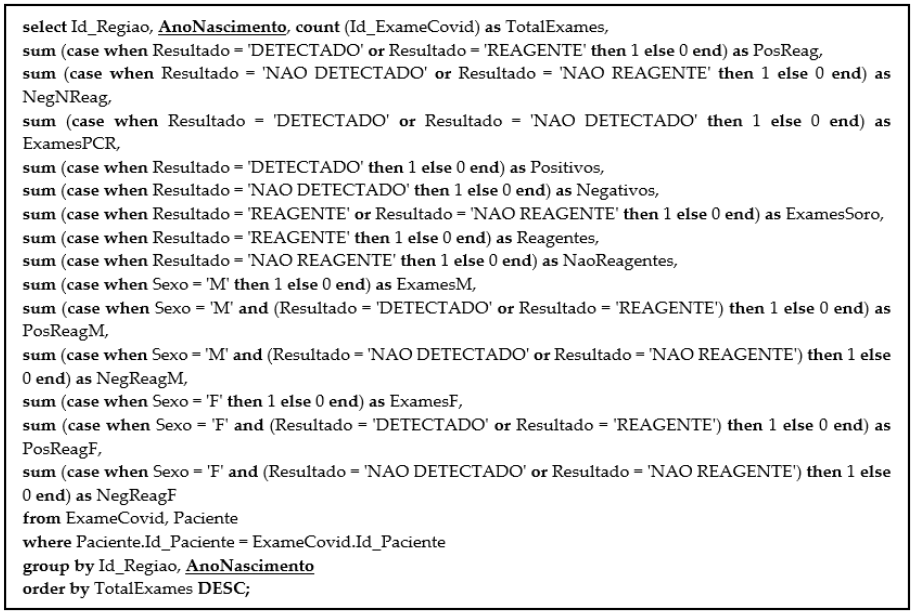
\includegraphics[width=0.85\textwidth]{figs/cov19-query12.png}
        \caption{Query Region (Query 1 - sin subrayado) y Query RegionYear (Query 2)}
        \label{cov19-q12}
    \end{center}
\end{figure}

\vspace{-0.5cm}

Por ejemplo, con la Consulta 1 Fig. \ref{cov19-q12}, MongoDB presenta los mejores resultados (1.76s) en comparación con SQL Server (2.59s) y Cassandra (7.14s), utilizando el conjunto de datos más pequeño. Estos tiempos se deben a que MongoDB es una base de datos distribuida por defecto, lo que permite una escalabilidad horizontal sin ningún cambio en la lógica de la aplicación. Analizando la escalabilidad de la base de datos cuando el tamaño se incrementa dos veces, los autores esperaban un aumento lineal en el tiempo de ejecución. Sin embargo, todas las bases de datos mostraron una buena escalabilidad, presentando un aumento en el tiempo de ejecución de solo 1.99 (MongoDB), 1.49 (SQL Server) y 1.12 (Cassandra). En este caso, concluyen que todas las bases de datos funcionan bien cuando aumentamos la carga de trabajo. Los resultados de la Consulta 2 son similares, con solo un aumento insignificante en el tiempo de ejecución de todas las bases de datos debido a la suma.

\begin{figure}[H]
    \centering
    \begin{minipage}[b]{0.48\textwidth}
        \centering
        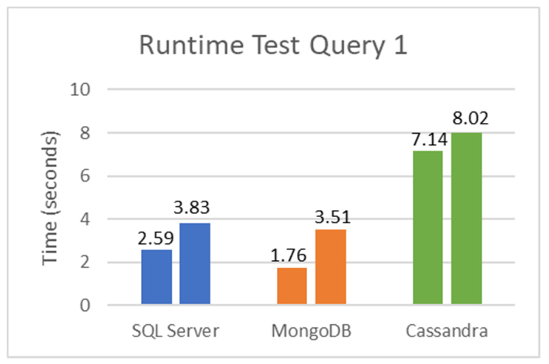
\includegraphics[width=\textwidth]{figs/cov19-runt-test-q1.png}
        \caption{Prueba de tiempo de ejecución para la Consulta 1.}
    \end{minipage}
    \hfill
    \begin{minipage}[b]{0.48\textwidth}
        \centering
        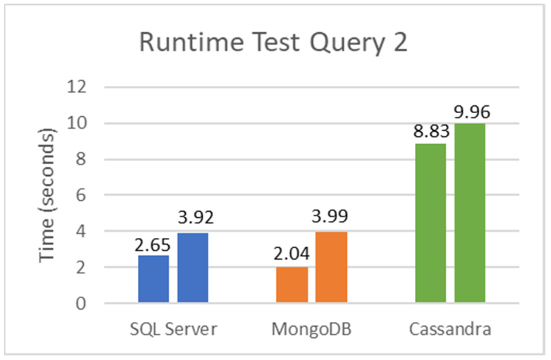
\includegraphics[width=\textwidth]{figs/cov19-runt-test-q2.png}
        \caption{Prueba de tiempo de ejecución para la Consulta 2.}
    \end{minipage}
\end{figure}

\vspace{-0.5cm}

La Fig. \ref{cov19-memtest-q1} y  Fig. \ref{cov19-memtest-q2} muestran el uso de RAM para la Consulta 1 y la Consulta 2 durante la ejecución en diferentes bases de datos. SQL Server utilizó menos memoria que MongoDB y Cassandra en ambas consultas. En cuanto a MongoDB, la diferencia va desde un mínimo de 101.6 MB hasta un máximo de 238.11 MB. Esta diferencia es marginal con Cassandra, donde la diferencia mínima es de 73.1 MB y la máxima es de 111.7 MB en comparación con el uso de RAM de SQL Server. Esto podría deberse al uso de replicación de datos por parte de MongoDB y Cassandra.

\begin{figure}[H]
    \centering
    \begin{minipage}[b]{0.48\textwidth}
        \centering
        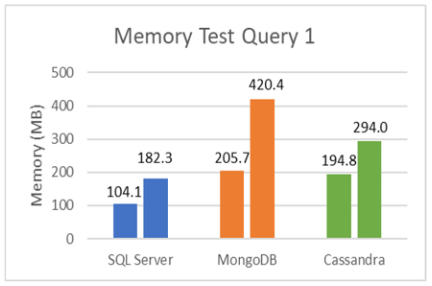
\includegraphics[width=\textwidth]{figs/cov19-mem-test-q1.png}
        \caption{Memoria RAM utilizada para la Consulta 1.}
        \label{cov19-memtest-q1}
    \end{minipage}
    \hfill
    \begin{minipage}[b]{0.48\textwidth}
        \centering
        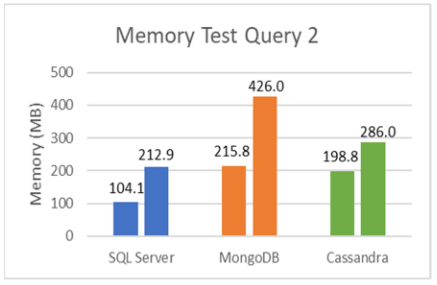
\includegraphics[width=\textwidth]{figs/cov19-mem-test-q2.png}
        \caption{Memoria RAM utilizada para la Consulta 2.}
        \label{cov19-memtest-q2}
    \end{minipage}
\end{figure}

\vspace{-0.5cm}

La Fig. \ref{cov19-cputest-q1} y Fig. \ref{cov19-cputest-q2} muestran el porcentaje de uso de CPU para la Consulta 1 y la Consulta 2, respectivamente, durante su ejecución en las diferentes bases de datos. Se observó que SQL Server utiliza menos CPU que MongoDB y Cassandra al ejecutar ambas consultas, con una diferencia máxima de 1.19× y 4.78×, respectivamente.

\begin{figure}[H]
    \centering
    \begin{minipage}[b]{0.48\textwidth}
        \centering
        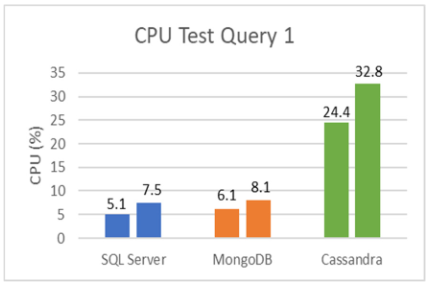
\includegraphics[width=\textwidth]{figs/cov19-cpu-test-q1.png}
        \caption{Porcentaje de CPU utilizado para la Consulta 1.}
        \label{cov19-cputest-q1}
    \end{minipage}
    \hfill
    \begin{minipage}[b]{0.48\textwidth}
        \centering
        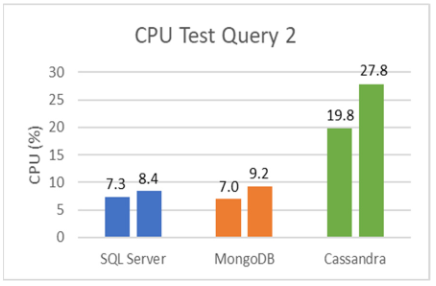
\includegraphics[width=\textwidth]{figs/cov19-cpu-test-q2.png}
        \caption{Porcentaje de CPU utilizado para la Consulta 2.}
        \label{cov19-cputest-q2}
    \end{minipage}
\end{figure}

\vspace{-0.5cm}

La tercera consulta Fig. \ref{cov19-q3} fue seleccionada utilizando un registro de auditoría activado que controlaba todas las consultas realizadas en la base de datos de SQL Server. Cuando Orange Data Mining estaba conectado a SQL Server, y se realizaron las pruebas de Minería de Datos (pruebas de clasificación), el registro de auditoría controlaba todas las consultas que Orange necesitaba realizar en la base de datos para realizar las pruebas. Por lo tanto, la tercera consulta evaluada fue la consulta que mostró el registro de auditoría. Esta consulta muestra el número de registros en la tabla \textit{SymptomsCovid}.

\vspace{-0.5cm}

\begin{figure}[H]
    \begin{center}
        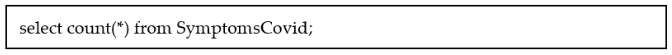
\includegraphics[width=0.82\textwidth]{figs/cov19-query3.png}
        \caption{Query Orange (Query 3)}
        \label{cov19-q3}
    \end{center}
\end{figure}

\vspace{-0.6cm}

Las Figs. \ref{cov19-runtest-q3}, \ref{cov19-memtest-q3} y y \ref{cov19-cputest-q3} muestran los resultados de la Consulta 3 durante su ejecución utilizando las diferentes bases de datos. La escalabilidad se evaluó utilizando \textit{SymptomsCovid} con 1,510,722 registros en la primera prueba y 3,021,444 registros en la segunda prueba. Los resultados de la Fig. \ref{cov19-runtest-q3} muestran que MongoDB y Cassandra fueron mucho mejores que SQL Server en tiempo de ejecución como se esperaba, ya que las bases de datos NoSQL se basan en la desnormalización y tratan de optimizar para el caso desnormalizado. Este factor hace que las consultas sean mucho más rápidas porque los datos se almacenan en el mismo lugar (tabla o colección), y no hay necesidad de realizar un \textit{join}. El modelo relacional utilizado por SQL Server resulta ser bastante perjudicial para este tipo de consultas.

En la Fig. \ref{cov19-memtest-q3} se muestra que SQL Server es la base de datos que utiliza más memoria para esta consulta. 

Finalmente, según la Figura \ref{cov19-cputest-q3}, ninguna de las bases de datos utiliza mucho CPU (\%) para ejecutar esta consulta, excepto Cassandra.

\begin{figure}[H]
    \centering
    \begin{minipage}[b]{0.48\textwidth}
        \centering
        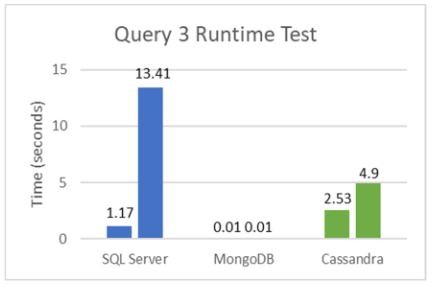
\includegraphics[width=\textwidth]{figs/cov19-runt-test-q3.png}
        \caption{Prueba de tiempo de ejecución para la Consulta 3.}
        \label{cov19-runtest-q3}
    \end{minipage}
    \hfill
    \begin{minipage}[b]{0.48\textwidth}
        \centering
        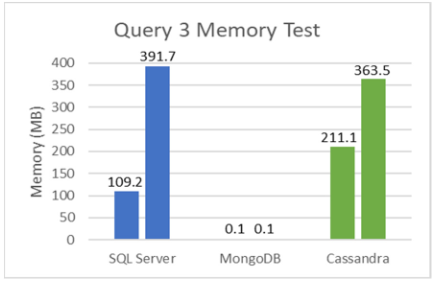
\includegraphics[width=\textwidth]{figs/cov19-mem-test-q3.png}
        \caption{Porcentaje de CPU utilizado para la Consulta 3.}
        \label{cov19-memtest-q3}
    \end{minipage}
\end{figure}

\vspace{-0.8cm}

\begin{figure}[H]
    \centering
    \begin{minipage}[b]{0.48\textwidth}
        \centering
        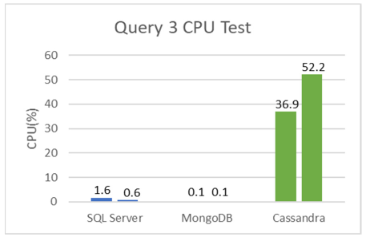
\includegraphics[width=\textwidth]{figs/cov19-cpu-test-q3.png}
        \caption{Porcentaje de CPU utilizado para la Consulta 3 .}
        \label{cov19-cputest-q3}
    \end{minipage}
    \hfill
    \begin{minipage}[b]{0.48\textwidth}
        \centering
        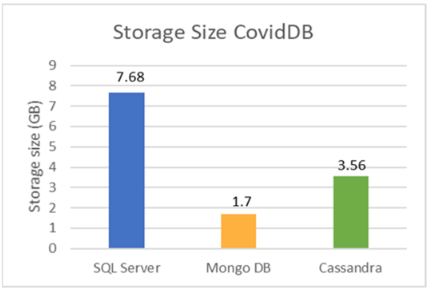
\includegraphics[width=\textwidth]{figs/cov19-storage.png}
        \caption{Tamaño de la base de datos de COVID-19.}
        \label{cov19-storage}
    \end{minipage}
\end{figure}

\vspace{-0.5cm}

Para terminar, se presenta la Fig. \ref{cov19-storage} la cuál muestra el tamaño de las tres bases de datos en GB.

Cabe destacar que los tres experimentos que no se mostraron, utilizaron consultas mas complejas, con \textit{joins}, y SQL Server tuvo un mejor rendimiento en general. 

\subsubsection{Conclusión de los Autores}\label{sec512}

Con respecto a este experimento, los autores concluyen que SQL Server debería ser la elección si los datos son muy estructurados y necesitan consultas con \textit{joins}. Cassandra y MongoDB mostraron un peor rendimiento con este tipo de consultas.

Sin embargo, si se utiliza un gran volumen de datos no estructurados y no es necesario realizar consultas de unión, MongoDB o Cassandra se consideran las soluciones más adecuadas. Para las consultas utilizadas, MongoDB fue más rápido y utilizó un porcentaje de CPU y tamaño de almacenamiento menor que Cassandra. Por otro lado, Cassandra fue la mejor en cuanto al uso de memoria. 

En última instancia, su elección sería MongoDB. Analizando la escalabilidad, las bases de datos NoSQL muestran un rendimiento superior al SQL Server, demostrando que son más apropiadas para procesar grandes cantidades de datos. 

\subsection{Performance investigation of selected SQL and NoSQL databases}\label{sec52}

Este artículo\cite{geo2015}, presentado en la Conferencia internacional sobre ciencia de la información geográfica (AGILE) por tres investigadores de la \textit{Universidad de Bundeswehr} en el año 2015:

\begin{center}
    Stephan Schmid, Eszter Galicz y Wolfgang Reinhardt.
\end{center}

Trata sobre la creciente importancia de los datos, especialmente los datos espaciales, en el mundo actual de alta tecnología. Se enfoca en la utilización de bases de datos como una forma efectiva de almacenar estos datos. Se menciona que, aunque las bases de datos relacionales son comúnmente utilizadas y funcionan bien para datos espaciales y no espaciales, pueden tener limitaciones en situaciones de alto volumen de datos y cambios frecuentes, como en redes sociales como Facebook o Twitter. Para abordar estas limitaciones, se exploran las bases de datos NoSQL, que pueden ser más adecuadas para grandes cantidades de datos y cambios frecuentes.

Las bases de datos utilizadas para este experimento fueron PostgreSQL, MongoDB Y CouchBase.

Nos enfocaremos en la conexión entre datos espaciales y las bases de datos NoSQL, así como en los experimentos de rendimiento que involucran tanto bases de datos SQL como NoSQL con este tipo de datos.

\subsubsection{Bases de Datos NoSQL sobre Geo-Aplicaciones}\label{sec521}

Dentro de las Bases de Datos NoSQL, solo las bases de datos de documentos y las bases de datos de grafos se utilizan ampliamente para almacenar datos espaciales.

Este estudio se concentró en las bases de datos de documentos. Tanto MongoDB como CouchBase, ambas de código abierto, admiten la representación de datos geoespaciales.

Teniendo en cuenta que que estas bases de datos son documentales, los autores utilizaron el formato GeoJSON, claramente basado en JSON, utilizado para codificar una variedad de estructuras de datos geográficos.

Un documento GeoJSON puede representar \textbf{Geometrías} (Puntos, Polígonos, Colección de Geometrías, etc.), \textbf{Features} y \textbf{Coleciones de Features} \cite{geojson}.

Al utilizar las estructuras de datos GeoJSON, el enfoque sin esquemas tiene algunas restricciones. Sin embargo, la representación geográfica debe seguir la estructura GeoJSON para poder establecer un índice geoespacial en la información geográfica. La indexación es importante para acelerar el procesamiento de consultas.

MongoDB actualmente utiliza dos índices geoespaciales, 2d y 2dsphere\cite{mongodb2dsphere}. El índice 2d se utiliza para calcular distancias en una superficie plana. El índice 2dsphere calcula geometrías sobre una esfera similar a la tierra.

CouchBase admite la indexación de datos bidimensionales mediante un índice R-Tree\cite{couchbase}. Por lo tanto, CouchBase proporciona vistas espaciales que permiten una consulta geoespacial utilizando cajas delimitadoras.

Para la base de datos relacional PostgreSQL, hay una extensión especial disponible, PostGIS, para integrar varias geo-funciones\cite{post-gis}. 

MongoDB y CouchBase no tienen una extensión separada, pero admiten algunas geo-funciones.

\vspace{-0.4cm}

\begin{table}[h!]
    \centering
    \begin{tabular}{ |c|c|c| }
    \hline
    PostGIS (selection)  & MongoDB & CouchBase \\ 
    \hline
    ST\_Within & \$geoWithin & BBOX \\
    ST\_Intersects & \$geoIntersects & \\ 
    & \$near &  \\
    ST\_Area & & \\
    ...& & \\
    \hline
    \end{tabular}
    \caption{Geo-Funciones de las bases de datos estudiadas.}
\end{table}

\vspace{-1cm}

\subsubsection{Experimentos sobre Bases de Datos}\label{sec522}

Para los experimentos, los autores utilizaron una computadora con las siguientes características:

\begin{itemize}
    \item Microsoft Windows Server 2008 R2
    \item 8 core CPU 2,5 GHz
    \item 10GB RAM
\end{itemize}

Los datos fueron obtenidos OpenStreetMap con diferentes tamaños, y fueron importados a las bases de datos. Se presenta más información en la siguiente tabla:

\begin{table}[h]
    \centering
    \begin{tabular}{ |c|c|c| }
    \hline
    Level & Region & Size \\ 
    \hline
    Subregion & Niederbayern & 38.9 MB \\
    State & Bayern & 501 MB \\ 
    Country & Germany & 2.1 GB \\
    \hline
    \end{tabular}
    \caption{Datos de prueba utilizados de OpenStreetMap.}
\end{table}

\vspace{-0.7cm}

Se utilizaron dos tipos de consultas para el análisis:

\begin{enumerate}
    \item Consultas sobre información de atributos: Se selecciona una característica de cada tipo de geometría (punto, línea y polígono) en función de su atributo (OSM\_id). Por ejemplo, de todos los objetos de punto se selecciona el punto con el OSM\_ID=1082817686.

    \begin{verbatim}
    Select * from points WHERE osm_id = '1082817686'
    \end{verbatim}

    \vspace{-0.4cm}
    
    \item La segunda consulta utiliza la geo-función '\textit{within}' para calcular datos a nivel de base de datos. Proporciona todos los puntos dentro del polígono definido. El polígono tiene el mismo tamaño para todas las solicitudes.

    \newpage
    
    \begin{verbatim}
    Select * from points WHERE
    (ST_Within (wkb_geometry, ST_GeomFromGeoJSON('
        {
        "type": "Polygon",
        "coordinates": [
            [[12.782592773437498,
            48.38817819201506 ],
            [12.782592773437498,
            48.54843286654265,
            [13.1231689453125,
            48.54843286654265],
            [13.1231689453125,
            48.38817819201506],
            [12.782592773437498,
            48.38817819201506]]],
        "crs": {
            "type": "name",
            "properties": {
            "name": "EPSG:4326" } 
            } 
        ]
    ')) is true)
    \end{verbatim}
\end{enumerate}

Para realizar la simulación en condiciones realistas, las consultas se realizaron con una determinada cantidad de usuarios, la cuál va en aumento. Las tres categorías de usuarios definidas fueron:

\begin{itemize}
    \item 100 usuarios.
    \item 250 usuarios.
    \item 500 usuarios.
\end{itemize}

\begin{wrapfigure}{r}{0.42\textwidth}
    \centering
    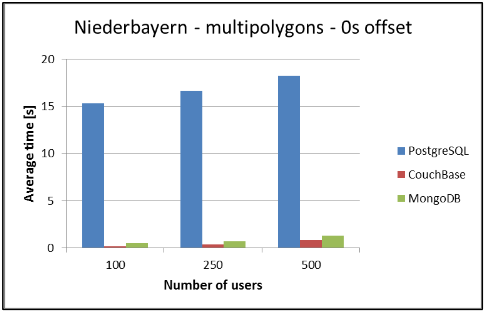
\includegraphics[width=0.5\textwidth]{figs/geo-g1.png}
    \caption{Consultas de información de atributos de multipolígonos.}
    \label{geo-g1}
\end{wrapfigure}

La Fig. \ref{geo-g1} muestra el tiempo de respuesta para solicitar información de atributos de un multipolígono. Compara las tres bases de datos probadas. Todas las pruebas se realizaron simultáneamente.

Queda claro que el tiempo de respuesta para el multipolígono de las bases de datos NoSQL es menor que para PostgreSQL. MongoDB y CouchBase se comportan casi de manera similar, aunque CouchBase es un poco más rápido.

Los autores mencionan que el experimento con la función \textit{within} sobre CouchBase no pudo llevarse a cabo por problemas con dicha implementación. La Fig. \ref{geo-g2} compara los resultados para MongoDB y PostgreSQL. El diagrama muestra los diferentes conjuntos de datos y tipos de geometría para 100 usuarios. Todas las solicitudes se realizaron al mismo tiempo.

\begin{wrapfigure}{r}{0.42\textwidth}
    \centering
    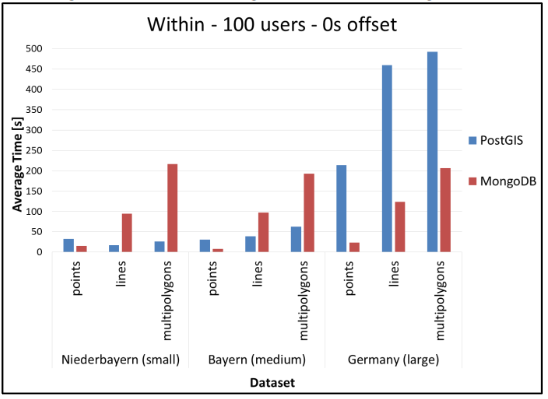
\includegraphics[width=0.5\textwidth]{figs/geo-g2.png}
    \caption{Consultas con geo-funciones en PostgreSQL y MongoDB.}
    \label{geo-g2}
\end{wrapfigure}

Para PostgreSQL (con tamaño de caché estándar), el tiempo de respuesta aumenta con el tamaño del conjunto de datos. Especialmente para el conjunto de datos grande (Alemania), el tiempo de respuesta alcanza los 200 segundos incluso para solicitudes en objetos de punto.

MongoDB se comporta de manera diferente. El tamaño del conjunto de datos no juega un papel importante. El tiempo de respuesta es casi lineal, solo difiere en algunos segundos.

PostgreSQL tiene un buen rendimiento independientemente del tipo de geometría en el conjunto de datos pequeño (Niederbayern). Eso cambia con un aumento en la cantidad de datos. Mientras que MongoDB mantiene el rendimiento incluso con conjuntos de datos grandes, el tiempo de respuesta de PostgreSQL aumenta rápidamente con el tamaño del conjunto de datos. Sin embargo, para conjuntos de datos pequeños, PostgreSQL funciona mejor cuando se consideran tipos de geometría complejos como líneas y multipolígonos.

\subsubsection{Conclusión de los Autores}\label{sec523}

En comparación directa con las pruebas de rendimiento de los dos casos de prueba, los resultados muestran que las consultas con el uso de geo-funciones llevan más tiempo que las consultas sobre información de atributos, lo cual era esperable. Para solicitudes puramente sobre información de atributos, las bases de datos NoSQL son muy rápidas y superiores en comparación con las bases de datos relacionales.

Para solicitudes con geo-funciones, las bases de datos NoSQL también tienen un rendimiento muy constante. Los tiempos de respuesta medidos varían solo unos pocos segundos para una cantidad creciente de datos. Pero para conjuntos de datos pequeños con geometría compleja, la base de datos relacional funcionó mejor.

MongoDB generalmente está optimizada para una configuración compartida en varios servidores. Esta posibilidad no se investigó en las pruebas, pero aún puede conducir a alguna mejora de rendimiento.

Los resultados presentados en el documento son válidos solo para la configuración de base de datos elegida, pero muestran claramente que las bases de datos NoSQL son una alternativa posible, al menos para consultar información de atributos.

\subsection{Conclusión}\label{sec53}

Nuestra conclusión sobre esta sección, coincide con la de los autores de ambos artículos y se alinea con lo expresado hasta el momento en nuestro propio estudio.

Como hemos mencionado, las bases de datos NoSQL son más adecuadas para el procesamiento de datos no estructurados y en grandes volúmenes, como se evidenció en ambos artículos. Sin embargo, debido a que tienen lenguajes de consulta menos potentes, las bases de datos SQL muestran un mejor rendimiento cuando se requieren consultas complejas.

Por lo tanto, antes de elegir una implementación específica, ya sea SQL o NoSQL, es importante considerar el tipo de problema que se está abordando, el tipo y tamaño de información que se manejará y las capacidades del hardware disponibles.

\section{Estado del arte}\label{sec6}

En este apartado examinamos el estado actual de las bases de datos NoSQL, analizando dos artículos recientes para mostrar algunos de los desafíos y enfoques que los investigadores de esta área están tomando. En particular se abordan:

\begin{enumerate}
    \item Aplicación de técnicas avanzadas de aprendizaje automático para mejorar la detección de fraudes en sistemas de bases de datos NoSQL.
    \item Utilización de las Bases de Datos de Grafo, en combinación con bases de datos ``tabulares" (SQL o NoSQL), para el almacenado de datos astronómicos y de experimentos de física de partículas.
\end{enumerate}

\subsection{Fraud Detection in NoSQL Database Systems
using Advanced Machine Learning}\label{sec61}

Las bases de datos NoSQL han transformado la manera en que las organizaciones gestionan grandes volúmenes de datos, proporcionando escalabilidad y flexibilidad superior a las bases de datos relacionales tradicionales. Sin embargo, esta evolución también ha traído consigo nuevos desafíos de seguridad. Este artículo\cite{fraud_detection}, escrito por Tamilselvan Arjunan y publicado en la revista \textit{International Journal of Innovative Science and Research Technology} en marzo de 2024, examina cómo el aprendizaje automatizado puede mejorar la detección de fraudes en sistemas de bases de datos NoSQL como \textit{MongoDB} y \textit{Cassandra}. Este trabajo destaca la vulnerabilidad de estos sistemas debido a sus esquemas dinámicos y la falta de control de acceso robusto, proponiendo el uso de algoritmos de aprendizaje automático para identificar comportamientos anómalos y no autorizados.

\subsubsection{Problemas de Seguridad en bases de datos NoSQL}
Las bases de datos NoSQL son conocidas por su flexibilidad en los esquemas de datos, lo cual permite adaptarse fácilmente a cambios en la estructura de los datos sin requerir modificaciones extensas en el esquema de la base de datos. Sin embargo, esta flexibilidad puede ser una espada de doble filo en términos de seguridad. Al no tener un esquema fijo y predefinido, resulta más complicado imponer restricciones y validaciones de datos de manera efectiva. Esto puede dar lugar a la inserción de datos maliciosos o no autorizados, lo que potencialmente compromete la integridad y la seguridad de los datos almacenados.

Por otro lado, muchos sistemas NoSQL, como \textit{Redis}, carecen de mecanismos nativos de control de acceso robustos. Esto significa que no hay una manera efectiva de gestionar quién tiene acceso a qué datos dentro del sistema. La falta de un control de acceso adecuado puede permitir que usuarios no autorizados accedan a datos sensibles o realicen modificaciones no autorizadas en la base de datos.

Además, estos sistemas a menudo adoptan modelos de consistencia eventual en lugar de consistencia fuerte. Si bien esto puede mejorar la disponibilidad y el rendimiento del sistema al permitir transacciones parcialmente completas, también introduce el riesgo de estados temporales inconsistentes. Esto significa que durante un período de tiempo, los datos pueden encontrarse en un estado intermedio o incompleto, lo que dificulta garantizar la integridad de los datos y puede ser aprovechado por atacantes para llevar a cabo acciones maliciosas.

Otro aspecto a considerar es la desnormalización de datos, común en las bases de datos NoSQL para evitar operaciones de join costosas en consultas. Sin embargo, esto puede resultar en la redundancia de datos y en una mayor exposición de información sensible. Al tener los datos desnormalizados, es más difícil controlar quién tiene acceso a qué datos y puede aumentar el riesgo de accesos no autorizados, especialmente si se combinan con la falta de controles de acceso adecuados.

Finalmente, muchos sistemas vienen con configuraciones predeterminadas que carecen de medidas básicas de seguridad, como cifrado de datos y autenticación sólida. Esto significa que, si los administradores no ajustan las configuraciones de seguridad, el sistema queda vulnerable a ataques. Los atacantes pueden aprovecharse de estas configuraciones por defecto para acceder fácilmente a los datos almacenados en la base de datos sin necesidad de autenticación, lo que representa un grave riesgo para la seguridad de la información.

\subsubsection{Soluciones Propuestas}

El monitoreo en tiempo real es esencial para identificar y responder rápidamente a amenazas en sistemas de bases de datos NoSQL. Al analizar continuamente los registros de la base de datos y las métricas de uso, se pueden detectar actividades anómalas y potencialmente maliciosas, lo que permite tomar medidas preventivas de manera oportuna.

Los algoritmos de aprendizaje automático ofrecen un enfoque poderoso para mejorar la detección de amenazas en sistemas NoSQL. Los modelos supervisados, como SVM, redes neuronales y bosques aleatorios, son entrenados con ejemplos de patrones maliciosos conocidos, lo que les permite identificar comportamientos anómalos en la base de datos con alta precisión. Por otro lado, las técnicas no supervisadas, como autoencoders y clustering basado en densidad, pueden detectar anomalías en el tráfico normal de la base de datos sin necesidad de ejemplos etiquetados. Además, los métodos en línea que se actualizan continuamente permiten adaptarse a nuevas amenazas, ofreciendo una detección adaptativa en tiempo real.

La ingeniería de características juega un papel crucial al transformar registros brutos en series temporales de metadatos normalizados. Esto facilita la identificación de patrones anómalos y maliciosos por parte de los modelos de aprendizaje automático, lo que mejora su capacidad de detección y reduce la incidencia de falsos positivos.

La combinación de modelado offline de comportamientos conocidos con detección de anomalías en línea proporciona una protección robusta y adaptativa contra amenazas dinámicas. Este enfoque híbrido aprovecha lo mejor de ambos mundos, permitiendo una detección eficaz tanto de amenazas conocidas como desconocidas.

Los proveedores deben integrar pipelines de aprendizaje automático embebidos en los sistemas NoSQL, equilibrando precisión y rendimiento. Además, es crucial asegurar que los modelos de Intrusion Detection Systems (IDS) se integren de manera efectiva con los flujos de trabajo de monitoreo y respuesta a amenazas para una protección completa.

Finalmente, incorporar técnicas de aprendizaje adversarial es esencial para mejorar la robustez de los modelos frente a intentos de evasión por parte de los atacantes. Esto garantiza una defensa más sólida contra amenazas potenciales y aumenta la eficacia general del sistema de detección de amenazas en entornos NoSQL.

\subsubsection{Conclusiones}

El uso de técnicas avanzadas de aprendizaje automático ofrece una solución prometedora para abordar los problemas de seguridad en las bases de datos NoSQL. Los modelos de machine learning tienen la capacidad de identificar comportamientos anómalos y no autorizados con alta precisión, proporcionando una capa adicional de seguridad que se adapta continuamente a nuevas amenazas.

Sin embargo, la implementación efectiva de estas técnicas en entornos de producción implica superar varios desafíos. Esto incluye la integración con sistemas existentes y la necesidad de datos etiquetados para el entrenamiento de los modelos. Además, es esencial que los proveedores y las organizaciones colaboren estrechamente para asegurar que las medidas de protección sean efectivas sin comprometer el rendimiento del sistema.

Para abordar estos desafíos y mejorar la seguridad en entornos NoSQL, se proponen las siguientes recomendaciones:

\begin{itemize}

    \item Integración de Machine Learning: Las organizaciones deben invertir en la integración de técnicas de aprendizaje automático en sus sistemas NoSQL para una detección y mitigación proactiva de amenazas.

    \item Fortalecimiento del Control de Acceso: Es crucial mejorar los mecanismos de control de acceso y autenticación para reducir la superficie de ataque y proteger los datos sensibles.

    \item Monitoreo y Auditoría: Establecer sistemas robustos de monitoreo y auditoría es fundamental para rastrear y responder eficientemente a actividades sospechosas, lo que permite una detección temprana de posibles amenazas.

    \item Actualización Continua: Mantener los modelos de detección de intrusiones actualizados es esencial para adaptarse a las técnicas de ataque en evolución. Esto incluye el uso de enfoques de aprendizaje adversarial para mejorar la robustez de los modelos.

    \item Colaboración Interdisciplinaria: Fomentar la colaboración entre equipos de desarrollo y seguridad es clave para asegurar la implementación efectiva de medidas de protección. Esta colaboración garantiza que se aborden los aspectos técnicos y de seguridad de manera integral, mejorando la postura general de seguridad de la organización.    
    
\end{itemize}

           
\subsection{The Future of the data storage in Particle Physics and Astronomy}\label{sec62}

Este artículo \cite{multidb}, desarrollado por Julius Hřivnáč y Julien Peloton, dos investigadores de la Université Paris-Saclay, en el año 2024, aborda cómo los experimentos de física de partículas y los telescopios de astronomía almacenan grandes cantidades de datos, principalmente en archivos simples en diversos formatos, con un uso limitado de bases de datos. A pesar de los avances en tecnología de bases de datos, estas posibilidades están subutilizadas. El artículo muestra de manera transparente la arquitectura de datos utilizando bases de datos ``tabulares" (SQL o NoSQL) y de Grafo, discutiendo sus fortalezas y debilidades, y describe formas de organizar la interacción entre ellas. Esto se ilustra con la implementación del \textbf{proyecto FINK}, del cuál ambos investigadores son parte, y que utiliza \textbf{HBase} y \textbf{JanusGraph} para almacenar alertas del Observatorio Rubin y del Zwicky Transient Facility. Utilizan HBase para almacenar datos voluminosos y JanusGraph para almacenar información estructural. También se esbozan formas de implementar arquitecturas de bases de datos heterogéneas en aplicaciones de física de partículas de alta energía en general.

\subsubsection{HEP Data}

En la Física de Alta Energía (HEP, por sus siglas en inglés), el manejo de datos ha dependido durante mucho tiempo de estructuras de datos convencionales. Estas incluyen tuplas, tablas y datagramas, así como estructuras más complejas como árboles y tuplas anidadas.

Sin embargo, una parte significativa de los datos de Física de Alta Energía exhibe características similares a grafos y carece de un esquema rígido. Estos datos a menudo consisten en entidades interconectadas a través de relaciones intrincadas, lo que los hace poco adecuados para el almacenamiento estándar en bases de datos relacionales convencionales.

Para abordar esto, se requiere un cambio fundamental. En lugar de tener un esquema predefinido fijo o manejar las relaciones externamente, es necesario permitir un manejo dinámico de la relación entre los elementos de los datos.

Sin embargo, este enfoque presenta su propio conjunto de desafíos. Las bases de datos relacionales tradicionales, que sobresalen en el manejo de relaciones bien definidas, luchan al enfrentarse con relaciones dinámicas y en evolución. Las bases de datos orientadas a objetos y los métodos de serialización también son insuficientes para manejar efectivamente estos datos, ya que tienen dificultades para distinguir relaciones esenciales de las volátiles.

\subsubsection{Performance de Bases de Datos en Grafo}

Las solicitudes en el contexto de la recuperación de datos en una base de datos de grafos generalmente atraviesan tres fases distintas:

\begin{itemize}
    \item \textbf{Búsqueda del Punto de Entrada Inicial:} La primera fase implica la búsqueda de un punto de entrada inicial dentro del conjunto de datos. Esta fase tiene potencial para optimización, a menudo beneficiándose de un orden natural, indexación y tecnologías como \textit{Elasticsearch} o \textit{Apache Spark} para mejorar la eficiencia de esta búsqueda inicial.
    
    \item \textbf{Navegación Jerárquica:} Esta fase implica una exploración más jerárquica del grafo de datos. Se caracteriza por un acceso muy rápido a datos interconectados, a menudo facilitado por las capacidades de la base de datos de grafos. Esta etapa permite un recorrido eficiente de las relaciones y la exploración de nodos de datos relacionados.
    
    \item \textbf{Acumulación de Resultados:} La fase final se preocupa por acumular y procesar los resultados obtenidos durante la fase de navegación.
\end{itemize}

Aunque las bases de datos de grafos ofrecen ventajas únicas, también presentan su propio conjunto de desafíos y limitaciones que deben ser considerados:

\begin{itemize}
    \item \textbf{Inserción Lenta}
    
    \item \textbf{Manejo de Memoria Lento}

    \item \textbf{Creación de Aristas Anárquica}
        
    \item \textbf{Esquema Desconocido y Relaciones Caóticas}
    
    \item \textbf{Lenguajes de Consulta Avanzados} 

    \item \textbf{etc.}
\end{itemize}

\subsubsection{Solución Hibrida}

En busca de un enfoque efectivo y versátil para la gestión de datos, emerge una solución híbrida que ofrece lo mejor de ambos mundos al combinar las fortalezas de diferentes paradigmas de almacenamiento.

Esta solución híbrida comienza almacenando datos no estructurados o en bruto en tablas tradicionales, como bases de datos SQL o NoSQL. Estos sistemas se eligen por su idoneidad para el procesamiento intensivo y paralelo.

Los datos almacenados en estructuras tipo tabla pueden organizarse y accederse de manera que se asemeje a la simplicidad y la interpretabilidad de las APIs tipo datagrama. Esto significa que los usuarios pueden acceder y manipular los datos con relativa facilidad, como si estuvieran trabajando con paquetes de datos simples o mensajes directos.

Mientras que los datos en bruto permanecen en almacenamiento tipo tabla, la solución híbrida introduce el concepto de un grafo para expresar y gestionar estructuras de datos persistentes. Este grafo representa relaciones y conexiones complejas dentro de los datos.

Esta solución permite la adición de relaciones de grafo ad-hoc, volátiles a priori. Estas relaciones dinámicas pueden establecerse y modificarse según sea necesario, proporcionando flexibilidad para adaptarse a los requisitos cambiantes de los datos. Estas relaciones pueden incluso existir en grafos separados pero interconectados, sirviendo como ``áreas de juegos" o ``pizarras" para experimentación y exploración.

Crucialmente, la solución híbrida conecta todos estos componentes detrás de una API común.

En esencia, este enfoque híbrido ofrece una manera versátil de gestionar datos. Aprovecha la eficiencia del almacenamiento tipo tabla para datos en bruto y el poder expresivo de los grafos para representar y explorar relaciones complejas. Al conectar estos elementos con una API común, se permite a los usuarios navegar, consultar y analizar datos de una manera que se adapte a sus necesidades específicas, ya sea para datos estructurados y persistentes o para escenarios experimentales dinámicos.

\begin{figure}[H]
    \centering
    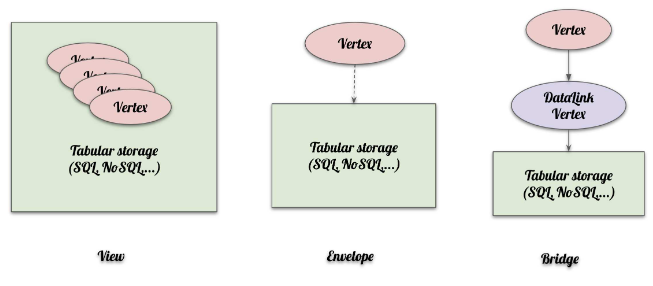
\includegraphics[width=0.9\textwidth]{figs/multidb-1.png}
    \caption{Tres arquitecturas para conectar bases de datos tabulares y de grafos en una solución híbrida. Tomado de \cite{multidb}.}
    \label{multidb-1}
\end{figure}

\begin{itemize}
    \item \textbf{Graph View:} El enfoque de ``Vista de Grafo" implica interpretar los datos tabulares existentes como vértices dentro de un grafo. Luego, se agregan aristas adicionales al grafo para expresar relaciones estructurales entre estos vértices. Sin embargo, implementar este enfoque puede ser desafiante. Para implementarlo efectivamente, se requiere una implementación completa y bastante genérica de un sistema de almacenamiento de grafos. Desarrollar este tipo de sistema puede ser complejo ya que implica traducir los datos tabulares existentes a un formato de grafo y garantizar la representación correcta de las relaciones.
    
    Cabe señalar que, aunque la mayoría de las implementaciones de bases de datos de grafos utilizan almacenamiento tabular como backend, a menudo imponen su propio esquema y mecanismos para manejar los datos del grafo.

    \item \textbf{Graph Envelope:} El enfoque de ``Envoltura de Grafo" implica mejorar el concepto de un vértice agregando métodos adicionales para llenarlo desde un almacenamiento tabular externo. Este enfoque ha sido implementado en algunos casos, sin embargo, viene con un conjunto de desafíos.
    
    Mantener la consistencia entre los datos almacenados dentro del vértice mejorado y los datos originales en el almacenamiento tabular externo puede ser complicado. Los cambios realizados en uno pueden no reflejarse inmediatamente en el otro. Determinar la semántica de búsqueda, como cómo se enrutan y ejecutan las consultas, puede ser complejo. Esto puede llevar a un rendimiento y comportamiento impredecibles. Los usuarios no siempre pueden estar conscientes de dónde reside realmente los datos y si se copiarán en el vértice mejorado o se accederán de forma remota. Esto puede afectar las decisiones de rendimiento y gestión de datos.
    
    \item \textbf{Bridge:} El enfoque ``Puente" implica la creación de un tipo especial de Vértice de Enlace de Datos que representa relaciones con datos externos almacenados en cualquier tipo de sistema de almacenamiento. Estos Vértices de Enlace de Datos pueden estar conectados a cualquier otro vértice en el grafo, formando efectivamente puentes hacia fuentes de datos externas. Este enfoque ofrece varias ventajas.
    
    Este enfoque es relativamente fácil de implementar en comparación con los otros dos enfoques. No requiere transformaciones de datos complejas ni cambios en el esquema. Proporciona una lógica transparente para conectar datos de diferentes fuentes. Los usuarios pueden trabajar con el grafo como si todos los datos estuvieran integrados sin problemas. Puede funcionar entre cualquier par de bases de datos con cualquier tecnología, incluida la conexión a otras bases de datos de grafos, lo que lo hace altamente versátil.

\end{itemize}

\subsubsection{Ejemplo de la vida real: \textit{FINK Project}}

El Observatorio Vera C. Rubin, hogar del Estudio del Legado del Espacio y del Tiempo (LSST) en Chile, emplea un telescopio de 8.4 metros y una cámara con una resolución de 3.2 gigapíxeles. Generará 10 millones de alertas cada noche, lo que equivale a aproximadamente 1 terabyte de datos de alerta con alrededor de 20 terabytes de datos de imagen. A lo largo de 10 años, se espera que LSST acumule alrededor de 60 petabytes de datos y aproximadamente 3 petabytes de datos de alerta\cite{lsstsciencecollaboration2009lsst}.
    
Las alertas producidas por LSST se diseminan globalmente a través de una red de ``brokers". Estos brokers desempeñan un papel crucial en la distribución y gestión de la vasta cantidad de datos de alerta generados por el observatorio.

El proyecto FINK\cite{fink} es reconocido como uno de los brokers oficiales dentro del Observatorio Rubin. Mientras este observatorio está en construcción, el broker FINK está recibiendo y analizando los datos del Zwicky Transient Facility (ZTF)\cite{zwicky}, que actúa como precursor utilizando tecnología similar para producir alertas. Desde 2019, ZTF está enviando en promedio 200,000 alertas por noche, y FINK está procesando y redistribuyendo estas alertas en tiempo real.
    
En este proyecto, todos los datos de alerta entrantes se almacenan sistemáticamente en tablas de Apache HBase. La estructura de los datos de alerta se crea y gestiona en JanusGraph, una potente base de datos de grafos\cite{janusgraph}. Esta estructura no solo contiene la relación con los datos principales, sino también los atributos más críticos asociados con cada alerta.

Un aspecto esencial de la gestión de datos en la arquitectura de almacenamiento de FINK es la presencia de enlaces de datos que conectan los datos en JanusGraph con los datos correspondientes en HBase. Estos enlaces de datos sirven como puentes entre los datos estructurados y orientados a grafos y los datos en bruto y tabulares almacenados en HBase, lo que permite un acceso y recuperación de información sin problemas.

En general, la combinación de HBase, JanusGraph y los enlaces de datos forma un sistema robusto de gestión de datos dentro de FINK, lo que permite un almacenamiento, organización y recuperación eficientes de los datos de alerta.

\begin{figure}[H]
    \centering
    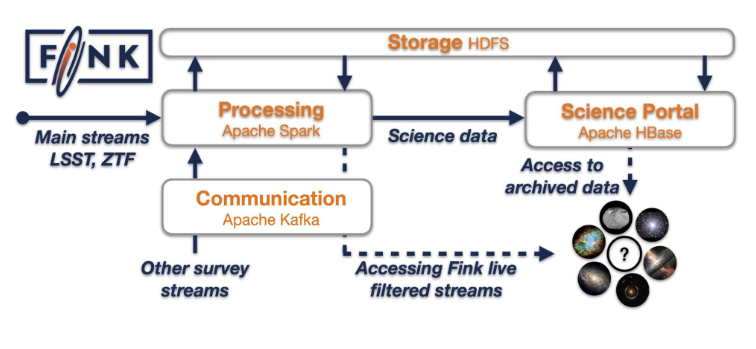
\includegraphics[width=0.9\textwidth]{figs/multidb-2.png}
    \caption{La arquitectura del broker FINK. Tomado de \cite{10.1093/mnras/staa3602}.}
    \label{multidb-2}
\end{figure}

Cada cuadro es un grupo de máquinas desplegadas en una nube. Los principales flujos de alertas para FINK (ZTF y LSST) se recogen y procesan dentro del clúster de Procesamiento que ejecuta Apache Spark. Al final del procesamiento, una serie de filtros divide el flujo en subflujos según las necesidades del usuario, y los datos se envían a los suscriptores a través del clúster de Comunicación que ejecuta Apache Kafka. Al final de la noche, todos los datos procesados se agregan y se envían al Portal de Ciencia, basado en Apache HBase, donde los usuarios pueden conectarse a través de un navegador web y explorar todos los datos procesados. Los datos de alertas y los valores añadidos se almacenan en varias etapas en el HDFS\cite{10.1093/mnras/staa3602}.

\subsubsection{Conclusiones}

El artículo destaca la importancia de estructurar los datos de manera efectiva en el contexto de la Física de Altas Energías (HEP) y las ventajas de utilizar bases de datos de grafos y soluciones de almacenamiento híbridas.

Las bases de datos de grafos ofrecen varias ventajas:

\begin{itemize}
    \item \textbf{Transparencia:} Hacen que el código sea más transparente al representar relaciones complejas de datos de manera intuitiva.
    
    \item Estructura de Datos Estable: La capa de almacenamiento maneja la estructura de datos, garantizando la estabilidad y consistencia de los datos.
    
    \item \textbf{Paralelismo:} Son adecuadas para el procesamiento paralelo, alineándose con las técnicas modernas de procesamiento de datos.
    
    \item \textbf{Análisis Declarativo:} Facilitan los análisis declarativos, donde las consultas describen qué recuperar, facilitando la comprensión y el procesamiento de datos.
    
    \item \textbf{Preservación del Análisis:} Pueden ayudar a preservar flujos de trabajo de análisis de datos, garantizando la reproducibilidad.
    
    \item \textbf{Neutralidad de Lenguaje y Marco de Trabajo:} Suelen ser neutrales en cuanto a lenguaje y marco de trabajo, lo que permite flexibilidad en la integración.
\end{itemize}

Las soluciones de almacenamiento híbridas combinan la expresividad y flexibilidad de las bases de datos de grafos con el rendimiento y la simplicidad del almacenamiento tabular, proporcionando lo mejor de ambos mundos. Una interfaz transparente facilita el trabajo con el almacenamiento híbrido, abstrayendo las complejidades.

Las bases de datos de grafos y las híbridas pueden mejorar la forma en que se manejan los datos en experimentos de Física de Altas Energías. Estas bases de datos facilitan la organización y comprensión de relaciones complejas dentro de los datos. Al combinar las fortalezas de múltiples tipos de bases de datos, los investigadores pueden gestionar los datos de manera más eficiente. Un ejemplo de la vida real utilizando el proyecto FINK demuestra los beneficios de utilizar estas tecnologías de bases de datos. Los enfoques descritos podrían mejorar la gestión de datos en experimentos de HEP.

\section{Integración de NoSQL en Diversos Contextos}\label{sec7}

En esta sección analizaremos las relaciones entre las bases de datos NoSQL con:

\begin{itemize}
    \item Espacios Métricos
    \item Bases de Datos Espacio-Temporales
    \item Web Semántica e \textit{Information Retrieval}
    \item Toma de Decisiones
\end{itemize}

Estos temas fueron presentados por compañeros en el curso de Bases de Datos Avanzadas.

\subsection{Espacios Métricos}

Los espacios métricos proporcionan estructuras matemáticas para definir distancias entre puntos, lo que permite medir similitudes y realizar búsquedas eficientes basadas en esas medidas. Esta herramienta es fundamental en áreas como la recuperación de información y el aprendizaje automático. Las bases de datos NoSQL, como MongoDB y Apache Cassandra, son ideales para manejar grandes volúmenes de datos y almacenar información en esquemas flexibles. Estas bases de datos pueden implementar estructuras de indexación específicas para manejar búsquedas en espacios métricos, permitiendo la organización y recuperación eficiente de datos basados en similitudes y distancias.

\subsection{Bases de Datos Espacio-Temporales}

Las bases de datos espacio-temporales son herramientas fundamentales que combinan la capacidad de almacenamiento de datos espaciales y temporales en un solo sistema, lo cual resulta esencial para diversas aplicaciones como sistemas de seguimiento, análisis climáticos y monitorización de eventos en tiempo real. Entre las soluciones destacadas en este campo se encuentra MongoDB, una base de datos NoSQL líder en el mercado que ofrece soporte nativo para índices geoespaciales y consultas de rango temporal. Esto permite gestionar eficazmente datos espacio-temporales en una única plataforma, facilitando la integración y el análisis de datos complejos.

\subsection{Web Semántica e \textit{Information Retrieval}}

La Web Semántica y la recuperación de información encuentran un aliado poderoso en las bases de datos NoSQL. Estas bases de datos ofrecen flexibilidad de esquema y capacidades avanzadas de indexación y búsqueda, lo que facilita el almacenamiento y consulta de datos semánticos. NoSQL es especialmente adecuado para la Web Semántica, ya que puede almacenar y consultar eficientemente datos semánticos, como grafos RDF. Además, puede soportar consultas semánticas complejas usando lenguajes de consulta intuitivos, lo que facilita la recuperación eficiente de información y abre nuevas posibilidades para la interoperabilidad de datos en la web.

\subsection{Toma de Decisiones}

La toma de decisiones se ve potenciada por las bases de datos NoSQL mediante tecnologías como \textit{Data Warehousing, Online Analytical Processing y Data Mining}. Estas herramientas permiten manejar grandes volúmenes de datos con flexibilidad de esquema y realizar análisis multidimensionales para una toma de decisiones más informada. En particular, MongoDB ofrece capacidades avanzadas de agregación y consultas complejas, lo que permite realizar análisis multidimensionales directamente sobre los datos almacenados. Esto facilita la creación de cubos \textit{OLAP} y agiliza el proceso de extracción de insights valiosos de los datos.

\section{Propuesta: Uso de Bases de Datos Multimodelo}\label{sec10}

\subsection{Introducción}

Las bases de datos multimodelo han surgido como una solución innovadora para gestionar y almacenar datos heterogéneos de manera eficiente. Estas bases de datos permiten manejar múltiples tipos de datos dentro de un único sistema de gestión, ofreciendo una flexibilidad y eficiencia sin precedentes. Se propone explorar las características, ventajas y desafíos de estas bases de datos, así como su aplicabilidad en diversos contextos empresariales.

\subsection{Objetivos}

El objetivo principal de esta investigación propuesta es comprender en profundidad las bases de datos multimodelo, identificando sus ventajas y desventajas en comparación con otros modelos de bases de datos tradicionales. Se propone evaluar su rendimiento en escenarios reales mediante estudios de caso y experimentos prácticos. Además, buscar desarrollar recomendaciones prácticas para su implementación y gestión efectiva en diferentes industrias.

\subsection{Metodología}

Para alcanzar los objetivos propuestos, se deberá realizar una revisión exhaustiva de la literatura existente sobre bases de datos multimodelo, analizando artículos académicos y estudios de caso relevantes. A continuación, se pueden identificar organizaciones que han adoptado estas bases de datos y evaluar su impacto en términos de eficiencia y gestión de datos. También, llevar a cabo pruebas empíricas utilizando bases de datos multimodelo populares, como ArangoDB y OrientDB, para así medir su rendimiento y capacidad de manejo de datos heterogéneos. Estos experimentos permitirán obtener datos concretos sobre su efectividad y posibles limitaciones.

\subsection{Resultados Esperados}

Se espera que esta investigación proporcione un marco conceptual claro para entender las bases de datos multimodelo y sus beneficios en comparación con los modelos tradicionales. Los resultados incluirían una identificación de las ventajas y limitaciones prácticas de estas bases de datos, así como recomendaciones para su implementación efectiva. Se anticipa que las bases de datos multimodelo demostrarán ser una solución viable y eficiente para la gestión de datos heterogéneos, optimizando las operaciones y mejorando la toma de decisiones en entornos complejos.


\section{Conclusiones}\label{sec9}

\begin{enumerate}
    \item \textbf{Popularidad y Ventajas de las Bases de Datos NoSQL.} Las bases de datos NoSQL han ganado una popularidad significativa en los últimos años, principalmente debido a su flexibilidad para manejar datos no estructurados o semiestructurados. Estas bases de datos son especialmente adecuadas para aplicaciones que requieren almacenar grandes volúmenes de datos y necesitan una estructura adaptable. Además, la escalabilidad de las bases de datos NoSQL es una de sus mayores fortalezas, permitiendo que las organizaciones crezcan y manejen cantidades masivas de información sin sacrificar el rendimiento. La facilidad de uso en entornos distribuidos también las convierte en una opción atractiva para muchas empresas que operan a nivel global y necesitan mantener una alta disponibilidad y resistencia ante fallos.
        
    \item \textbf{Complementariedad con las Bases de Datos Relacionales.} A pesar de sus numerosas ventajas, las bases de datos NoSQL no están diseñadas para reemplazar completamente a las bases de datos relacionales. Las bases de datos relacionales siguen siendo la mejor opción para gestionar datos estructurados que requieren relaciones complejas y cumplir con las propiedades ACID (Atomicidad, Consistencia, Aislamiento, Durabilidad). Estas características son cruciales para aplicaciones que necesitan transacciones confiables y coherentes, como sistemas financieros y de gestión empresarial. Por lo tanto, las bases de datos relacionales mantienen su relevancia en contextos donde la integridad de los datos y la consistencia transaccional son esenciales.
    
    \item \textbf{Propuestas de Hibridación entre Bases de Datos.} Existen propuestas sólidas que promueven la combinación de bases de datos NoSQL y relacionales, así como entre diferentes bases de datos NoSQL, sugiriendo que un enfoque híbrido puede ser altamente beneficioso. Esta estrategia permite a las organizaciones aprovechar las fortalezas de cada tipo de base de datos según el caso de uso específico. Por ejemplo, se pueden utilizar bases de datos relacionales para gestionar datos estructurados y transacciones críticas, mientras que las bases de datos NoSQL pueden manejar datos no estructurados y grandes volúmenes de información con flexibilidad y eficiencia. Este enfoque híbrido puede ofrecer una solución más robusta y versátil, optimizando el rendimiento y la capacidad de adaptación a diferentes necesidades.
    
    \item \textbf{Gran variedad de Implementaciones NoSQL.} La diversidad dentro del ecosistema de las bases de datos NoSQL es notable, con una amplia gama de implementaciones que ofrecen características y enfoques únicos. Esta variedad permite a las organizaciones seleccionar la solución más adecuada para cada caso de uso específico, desde bases de datos orientadas a documentos como MongoDB, hasta bases de datos clave-valor como Redis, y bases de datos orientadas a grafos como Neo4j. Cada tipo de base de datos NoSQL está diseñado para resolver problemas particulares, proporcionando opciones que pueden optimizar el manejo de datos y mejorar la eficiencia operativa en distintos contextos. Esta flexibilidad es crucial para desarrollar sistemas de gestión de datos que sean adaptables, escalables y alineados con los objetivos estratégicos de la organización.
\end{enumerate}

\newpage

\bibliography{referencias}\label{sec8}


\end{document}
